\documentclass[10pt,a4paper]{article}
\usepackage[utf8]{inputenc}
\usepackage[english,russian]{babel}
\usepackage{cmap}
\usepackage[OT1]{fontenc}
\usepackage{amsmath}
\usepackage{amsfonts}
\usepackage{amssymb}
\usepackage{graphicx}
\usepackage{float}
\usepackage{wrapfig}
\usepackage{caption}
\DeclareCaptionLabelSeparator{dot}{. }
\captionsetup{justification=centering,labelsep=dot}
\graphicspath{{pictures/}}
\DeclareGraphicsExtensions{.pdf,.png,.jpg,.eps}
\begin{document}



\textbf{13 Алгоритм FastSLAM}\\

Пришло время обратить внимание на метод \textit{многочастичного фильтра} в SLAM. Мы уже сталкивались с многочастичными фильтрами в нескольких главах книги и заметили, что они лежат в основе некоторых наиболее эффективных алгоритмов робототехники. Поэтому закономерно возникает вопрос применимости многочастичных фильтров для задачи SLAM. К сожалению, многочастичные фильтры подвержены «проклятью размерности»: там, где гауссовы фильтры требуют ресурсов, с зависимостью от линейной до квадратичной от числа измерений задачи оценки, сложность многочастичных фильтров возрастают экспоненциально! Прямолинейная реализация многочастичных фильтров для задачи SLAM обречена на провал, в силу большого числа переменных, используемых при описании карты.

Приведённый в этой главе алгоритм основан на важной характеристике задачи SLAM, которая ещё явно не обсуждалась в книге. Дело в том, что в задаче SLAM с известным соответствием соблюдается условная независимость между любыми двумя непересекающимися множествами признаков на карте, если задано положение робота. Другими словами, если некий оракул даст информацию об истинном положении робота, станет возможным оценить местоположение всех признаков независимо друг от друга. Зависимость в этих оценках возникает \textit{только} в силу неопределённости положения робота.\\

МНОГОЧАСТИЧНЫЙ ФИЛЬТР РАО-БЛЕКВЕЛЛА\\

Это структурное наблюдение делает возможным применение варианта многочастичного фильтра, известного под названием  \textit{многочастичный фильтр Рао-Блеквелла в SLAM}. Многочастичные фильтры Рао-Блеквелла выражают апостериорную вероятность по нескольким переменным, а также их гауссианам (или другим параметрическим функциями) для выражения всех прочих переменных.\\

УСЛОВНАЯ ВЕРОЯТНОСТЬ\\

В FastSLAM  многочастичные фильтры используется для оценки по пути робота. Как можно увидеть, для каждой из частиц ошибки отдельных карт \textit{условно независимы}, поэтому задачу картографирования можно разбить на множество отдельных задач, по одной для каждого признака на карте. FastSLAM оценивает местоположение этих признаков на карте с помощью EKF, используя отдельный EKF низкой размерности для каждого отдельного признака. Это сильно отличается от алгоритмов SLAM, обсуждаемых в прошлых главах, в которых всегда использовался один гауссиан для совокупной оценки всех признаков.

Основной алгоритм может быть реализован за время, логарифмически зависящее от числа признаков. Поэтому, FastSLAM имеет определённые вычислительные преимущества перед обычными реализациями EKF и многими из их вариаций. Ключевое преимущество FastSLAM, однако, проистекает из возможности выполнить решение ассоциации данных на основе отдельных частиц. В результате, в фильтре сохраняются апостериорные вероятности по нескольким ассоциациям данных, а не только по самой вероятной. Это полностью противоположно всем алгоритмам SLAM, которые до сих пор обсуждались, и в которых отслеживалась только одна ассоциация данных в произвольный момент времени. Фактически, выполняя выборку по ассоциациям данных, FastSLAM аппроксимирует полную апостериорную вероятность, а не только ассоциацию данных, имеющую максимальное правдоподобие. Эмпирически подтверждено, что возможность сохранять несколько ассоциаций данных одновременно делает FastSLAM существенно повышает устойчивость к проблемам ассоциации данных, по сравнению с алгоритмами инкрементной ассоциации данных по максимальному правдоподобию.

Другое преимущество FastSLAM по сравнению с другими алгоритмами SLAM возникает из-за того, что многочастичные фильтры могут справляться с нелинейными моделями движения робота, там, где предыдущие методы аппроксимировали такие модели с помощью линейных функций. Это важно при высокой нелинейности кинематики, или же, когда неопределённость положения сравнительно высока.

Использование многочастичных фильтров создаёт необычную ситуацию, когда алгоритм FastSLAM решает сразу и \textit{полную задачу SLAM}, и \textit{онлайновую задачу SLAM}. Как будет показано далее, FastSLAM сформулирован для вычисления полной апостериорной вероятности пути, поскольку только наличие полного пути обеспечивает местоположениям признаков условную независимость. Однако, поскольку многочастичные фильтры выполняют одну оценку за один проход, FastSLAM в действительности является онлайновым алгоритмом и также решает онлайн задачу SLAM. Среди всех обсуждаемых алгоритмов SLAM, FastSLAM является единственным алгоритмом, попадающим сразу в две категории.

В этой главе описано несколько версий алгоритма FastSLAM. FastSLAM 1.0 – это оригинальный алгоритм FastSLAM, который концептуально прост и лёгок в реализации. Но, в некоторых ситуациях, компонент многочастичного фильтра в FastSLAM 1.0 неэффективно генерирует выборку. В алгоритме FastSLAM 2.0 эта проблема решена улучшенным предполагаемым распределением, но ценою существенно более сложной реализации (как и математического вывода). В обоих алгоритмах FastSLAM используется модель датчика на основе признаков, обсуждаемая ранее. Применение FastSLAM для датчиков расстояния даст алгоритм, решающий задачу SLAM в контексте карт сетки занятости.  Для всех алгоритмов в этой главе приведены методы оценки переменных ассоциации данных.\\

\textbf{13.1	Основной алгоритм}\\

Частица в базовом алгоритме FastSLAM имеют вид, показанный в Таблице 13.1.  Каждая частица содержит оценку положения робота, обозначаемую $x_t^[k]$, и набор калмановских фильтров с математическим ожиданием $\mu_{j,t}^[k]$ и ковариацией $\varSigma_{j,t}^[k]$, по одному для каждого признака
$m_j$ на карте.  Здесь $[k]$ – индекс частицы, а общее количество частиц обозначим $M$, как уже делалось раньше.

Шаг обновления базового FastSLAM приведён в Таблице 13.2. За множеством различных деталей обновления скрывается основной цикл, практически идентичный многочастичному фильтру, обсуждаемому в Главе 4. Первый шаг включает извлечение частицы, выражающей апостериорную вероятность в момент времени $t-1$, и выборку значений положения робота в момент времени $t$ на основе вероятностной модели движения. На следующем шаге выполняется обновление EKF для наблюдаемых признаков, используя стандартное уравнение обновления EKF. Оно не является частью  первоначального многочастичного фильтра, но необходимо в FastSLAM для изучения карты. Последние операции связаны с вычислением веса значимости, который затем используется для перевыборки частиц.

Разберём каждый шаг более детально и выведем их из базовых математических свойств задачи SLAM. Остановимся на том, что вывод изначально предполагает, что FastSLAM решает полную задачу SLAM, а не только онлайновую. Однако, в ходе дальнейших рассуждений станет ясно, что FastSLAM является решением для обеих задач. Каждую частицу можно рассматривать в виде элемента выборки в пространстве путей, что требуется для полной задачи SLAM, но обновление требует наличия только текущего положения, поэтому можно запускать FastSLAM и в качестве фильтра.\\

\textbf{13.2	Факторизация апостериорной вероятности в SLAM }\\

Ключевая математическая идея FastSLAM относится к тому факту, что полная апостериорная вероятность SLAM, $p(y_{1:t}|z_{1:t},u_{1:t})$ в выражении (10.2) может быть переписана в виде множителей\\

(13.1)
$$p(y_{1:t}|z_{1:t},u_{1:t},c_{1:t})=p(x_{1:t}|z_{1:t},u_{1:t},c_{1:t})\prod_{n=1}^Np(m_n|x_{1:t},z_{1:t},c_{1:t})$$

\textit{Факторизация} определяет, что вычисление апостериорной вероятности по путям и картам может быть разложена на $N +1$ вероятностей.

\begin{figure}[H]
	\center{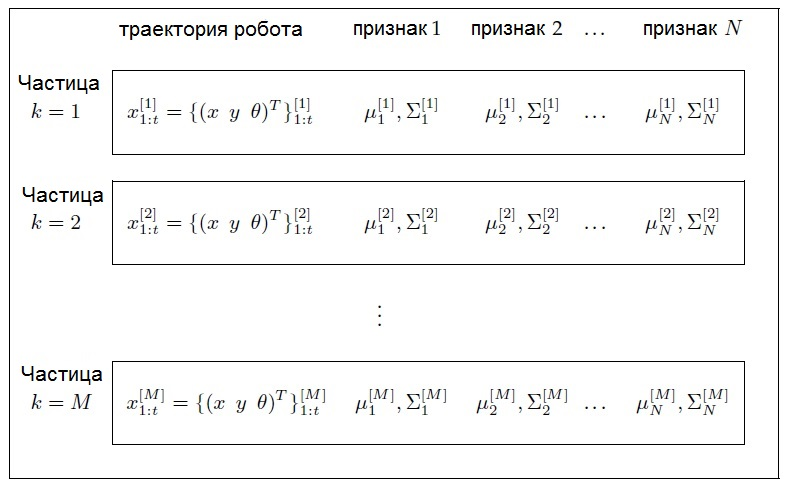
\includegraphics[width=1\linewidth]{131orig}}
	\caption{ ( Рис. 13.1 Частицы в FastSLAM состоят из оценки пути и набора оценивающих функций местоположений отдельных признаков со связанными с ними ковариациями.) }
	\label{fig:131orig}
\end{figure}

\begin{table}[H]
\begin{center}
\begin{tabular}{|l|}
\hline
{}\\
•	Выполнить следующие шаги $M$ раз:\\
{}\\
\hspace{3mm}–   \textbf{Извлечение.} Извлечь положение $x_{t-1}^{[k]}$   из набора частиц  $Y_{t-1}$.\\
{}\\
\hspace{3mm}–   \textbf{Прогноз}. Сделать выборку нового положения $x_t^{[k]}\sim p(x_t|x_{t-1}^{[k]},u_t)$.\\
{}\\
\hspace{3mm}–  \textbf{ Обновление измерения.}  Для каждого наблюдаемого признака $z_t^i$ \\
\hspace{8mm}определить соответствие $j$ измерения $z_t^i$, и учесть измерение $z_t^i$\\
\hspace{7mm}  в соответствующем EKF, обновив среднее $_{j,t}^{[k]}$  и ковариацию $\varSigma_{j,t}^{[k]}$\\
{}\\
\hspace{3mm}–   \textbf{Вес значимости}.  Вычислить вес значимости $w^{[k]}$ для новой частицы.\\
{}\\
•	\textbf{Перевыборка.} Выполнить выборку с заменой $M$ частиц, где каждая \\
\hspace{3mm}частица выбирается с вероятностью, пропорциональной $w^{[k]}$.\\
{}\\
\hline
\end{tabular}
\caption{(Рис. 13.2    Основные шаги алгоритма FastSLAM)}
\end{center}
\end{table}

\begin{figure}[H]
	\center{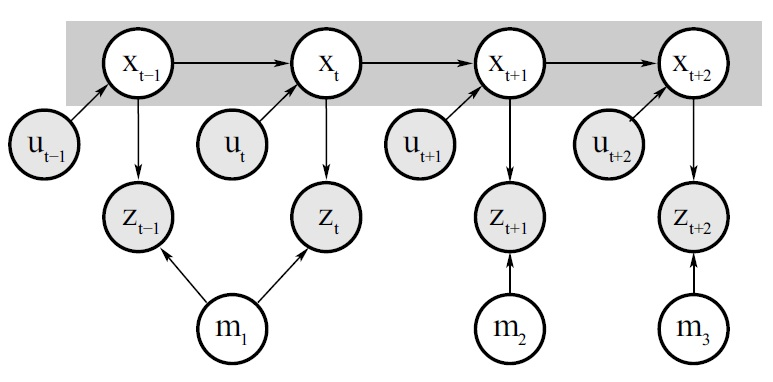
\includegraphics[width=0.8\linewidth]{133orig}}
	\caption{ ( Рис. 13.3 Задача SLAM в виде графа байесовской сети. Робот перемещается из положения $x_{t-1}$ в положение $x_{t+2}$, выполняя последовательность сигналов управления. В каждом положении $x_t$ наблюдается близлежащий признак на карте $m=\{m_1,m_2,m_3\}$. На этой графической сети показано, что переменная положения «разделяет» отдельные признаки на карте друг от друга. Если положения известны, между двумя признаками на карте не останется путей с неизвестными переменными. Отсутствие пути обуславливает условную независимость апостериорной вероятности любых двух признаков (при заданном положении).) }
	\label{fig:133orig}
\end{figure}

В FastSLAM используется многочастичный фильтр для вычисления апостериорного распределения по траекториям робота, обозначенную  $p(x_{1:t}| z_{1:t}, u_{1:t}, c_{1:t})$. Для каждого признака на карте в FastSLAM используются отдельные функции оценки по местонахождению $p(m_n|x_{1:t}, c_{1:t}, z_{1:t})$, для $n = 1,...,N$ . Поэтому, в сумме получится $N+1$ апостериорных вероятностей FastSLAM. Оценивающие функции признаков зависят от пути робота, что означает наличие отдельной копии для каждой функции оценки признака, по одной для каждой частицы. Для $M$ частиц количество фильтров будет равно $1+MN$. Произведение этих вероятностей выражает искомое апостериорное распределение в виде множителей. Как будет показано ниже, выражение в виде множителей является точным, а не просто приближением, что является общей характеристикой задачи SLAM.

Для иллюстрации корректности этой факторизации, на Рис. 13.3 графически показан процесс получения данных в виде динамической байесовской сети. Как подразумевает этот граф, каждое измерение $z_1,..., z_t$ является функцией соответствия признака, а также положения робота в момент времени, когда было выполнено измерение. Знание пути робота выделяет проблемы оценки отдельного признака и делает их независимыми друг от друга, в том смысле, что не существует прямого, в графическом выражении, пути от одного признака к другому, который бы не включал в себя переменных пути робота. Знание точного местонахождения одного признака, таким образом, ничего не скажет о местонахождении остальных признаков. Это указывает на \textit{условную независимость} признаков при заданном пути, как указано в выражении (13.1).

Перед обсуждением выводов на основе этого свойства задачи SLAM приведём краткий математический вывод.\\

\textbf{13.2.1	Математический вывод факторизованной апостериорной вероятности SLAM }\\

Выведем уравнение (13.1) из первых закономерностей. Очевидно, имеется\\

(13.2)
$$p(y_{1:t}|z_{1:t},u_{1:t},c_{1:t})=p(x_{1:t}|z_{1:t},u_{1:t},c_{1:t})\,p(m|x_{1:t},z_{1:t},c_{1:t})$$

Достаточно показать, что второй множитель с правой стороны можно выразить следующим образом:\\

(13.3)
$$p(m|x_{1:t},c_{1:t},z_{1:t})=\prod_{n=1}^Np(m_n|x_{1:t},c_{1:t},z_{1:t})$$

Докажем это методом индукции. Вывод потребует выделения двух возможных случаев, в зависимости от того, наблюдается ли признак $m_n$ в самом последнем измерении. В частности, если $c_t\neq n$, является самым последним измерением, $z_t$ не оказывает никакого эффекта на апостериорную вероятность, а также на положение робота $x_t$ или соответствие $c_t$. Отсюда, получим:\\

(13.4)
$$p(m_n|x_{1:t},c_{1:t},z_{1:t})=p(m_n|x_{1:t-1},c_{1:t-1},z_{1:t-1})$$

Если $c_t=n$, а  значит, и $m_n = m_{c_t}$ наблюдался в самом последнем измерении $z_t$, возможно применить теорему Байеса, с некоторыми стандартными упрощениями:\\

(13.5)
\begin{equation*}
\begin{split}
p(m_{c_t}|x_{1:t},c_{1:t},z_{1:t})&=\frac{p(z_t|m_{c_t},x_{1:t},c_{1:t},z_{1:t-1})p(m_{c_t}|x_{1:t},c_{1:t},z_{1:t-1})}{p(z_t|x_{1:t},c_{1:t},z_{1:t-1})}\\
&=\frac{p(z_t|x_t,m_{c_t},c_t)p(m_{c_t}|x_{1:t-1},c_{1:t-1},z_{1:t-1})}{p(z_t|x_{1:t},c_{1:t},z_{1:t-1})}
\end{split}
\end{equation*}

Это да`т следующее выражение для вероятности наблюдаемого признака $m_{c_t}$:\\

(13.6)
$$p(m_{c_t}|x_{1:t-1},c_{1:t-1},z_{1:t-1})=\frac{p(m_{c_t}|x_{1:t},c_{1:t},z_{1:t})p(z_t|x_{1:t},c_{1:t},z_{1:t-1})}{p(z_t|x_t,m_{c_t},c_t)}$$

Доказательство верности (13.3) выполняется через индукцию. Допустим, что апостериорная вероятность в момент времени $t-1$ уже факторизована:\\

(13.7)
$$p(m|x_{1:t-1},c_{1:t-1},z_{1:t-1})=\prod_{n=1}^Np(m_n|x_{1:t-1},c_{1:t-1},z_{1:t-1})$$

Это утверждение тривиально для $t=1$, поскольку в начальный момент у робота нет информации ни об одном признаке, а, значит, все оценки независимы. В момент времени $t$, апостериорная вероятность имеет следующий вид:\\

(13.8)
\begin{equation*}
\begin{split}
p(m_{c_t}|x_{1:t},c_{1:t},z_{1:t})&=\frac{p(z_t|m,x_{1:t},c_{1:t},z_{1:t-1})p(m|x_{1:t},c_{1:t},z_{1:t-1})}{p(z_t|x_{1:t},c_{1:t},z_{1:t-1})}\\
&=\frac{p(z_t|x_t,m_{c_t},c_t)p(m|x_{1:t-1},c_{1:t-1},z_{1:t-1})}{p(z_t|x_{1:t},c_{1:t},z_{1:t-1})}
\end{split}
\end{equation*}

Вставка этого выражения в гипотезу индукции (13.7) даст:\\

(13.9)
\begin{equation*}
\begin{split}
p(m&|x_{1:t},c_{1:t},z_{1:t})\\
&=\frac{p(z_t|x_t,m_{c_t},c_t)}{p(z_t|x_{1:t},c_{1:t},z_{1:t-1})}\prod_{n=1}^Np(m_n|x_{1:t-1},c_{1:t-1},z_{1:t-1})\\
&=\frac{p(z_t|x_t,m_{c_t},c_t)}{p(z_t|x_{1:t},c_{1:t},z_{1:t-1})}\underbrace{p(m_{c_t}|x_{1:t-1},c_{1:t-1},z_{1:t-1})}_{\text{форм. (13.6)}}\\
&\hspace{40mm}\prod_{n\neq c_t}\underbrace {p(m_n|x_{1:t-1},c_{1:t-1},z_{1:t-1})}_{\text{форм. (13.4)}}\\
&=p(m_{c_t}|x_{1:t},c_{1:t},z_{1:t})\prod_{n\neq c_t}p(m_n|x_{1:t},c_{1:t},z_{1:t})\\
&=\prod_{n=1}^Np(m_n|x_{1:t},c_{1:t},z_{1:t})
\end{split}
\end{equation*}

Заметим, что были заменены выражения (13.4) и (13.6), что показывает правильность выражения (13.3). Правильность основного вида выражения (13.1) напрямую следует из результата и последующего общего преобразования:\\

(13.10)
\begin{equation*}
\begin{split}
p(y_{1:t}|z_{1:t},u_{1:t},c_{1:t})&=p(x_{1:t}|z_{1:t},u_{1:t},c_{1:t})p(m|x_{1:t},z_{1:t},u_{1:t},c_{1:t})\\
&=p(x_{1:t}|z_{1:t},u_{1:t},c_{1:t})p(m|x_{1:t},c_{1:t},z_{1:t})\\
&=p(x_{1:t}|z_{1:t},u_{1:t},c_{1:t})\prod_{n=1}^Np(m_n|x_{1:t},c_{1:t},z_{1:t})
\end{split}
\end{equation*}

Заметим, что зависимость от всего пути $x_{1:t}$ действительно важна для результата. Зависимости от самого последнего положения $x_t$ может быть недостаточно для переменной зависимости, поскольку зависимости могут возникать из предыдущих положений робота.

\begin{figure}[H]
	\center{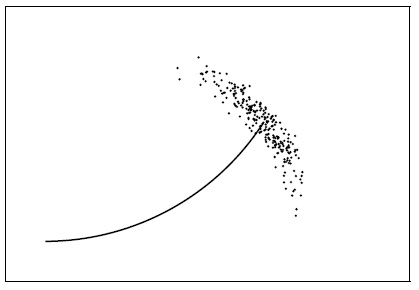
\includegraphics[width=0.5\linewidth]{134orig}}
	\caption{ ( Рис. 13.4   Выборка значений из вероятностной модели движения.) }
	\label{fig:134orig}
\end{figure}

\textbf{13.3	FastSLAM с известной ассоциацией данных}\\

Выражение апостериорной вероятности в виде множителей даёт существенные вычислительные преимущества над алгоритмами SLAM оценивающими неструктурированное апостериорное распределение. В FastSLAM используется факторизованное выражение в силу сохранения $MN +1$ фильтров, $M$ для каждого множителя в (13.1). В силу этого все $MN +1$ имеют малую размерность.

Как было отмечено, в FastSLAM оценивается апостериорная вероятность по пути робота с помощью многочастичного фильтра. Местоположения признака карты оцениваются, используя EKF. В силу факторизации, FastSLAM может сохранять отдельный фильтр EKF для каждого признака, что делает обновление более эффективным по сравнению с EKF SLAM. Каждый отдельный EKF зависит от пути робота, поэтому каждая частица имеет собственный набор значений. В общей сложности имеется $NM$ EKF, по одному для каждого признака на карте и по одному для каждой частицы многочастичного фильтра.
 
Начнём с алгоритма FastSLAM для известной ассоциации данных. Частицы в FastSLAM будут определены\\

(13.11)
$$Y_t^{[k]}=\langle x_t^{[k]},\mu_{1,t}^{[k]},\varSigma_{1,t}^{[k]},...,\mu_{N,t}^{[k]},\varSigma_{N,t}^{[k]}\rangle$$

Как обычно, квадратные скобки $[k]$ указывают на индекс частицы, $x_t^{[k]}$ это оценка пути робота, а $\mu_{n,t}^{[k]}$ и $\varSigma_{n,t}^{[k]}$ - математическая ожидание и дисперсия гауссового выражения местоположения $n$-го признака, относительно $k$-й частицы. Вместе все эти показатели образуют $k$-ю частицу $Y_t^{[k]}$, которых в апостериорном распределении FastSLAM имеется $M$.

Фильтрация, или апостериорное распределение в момент времени $t$ из такового в момент времени $t-1$, включает генерацию нового набора частиц $Y_t$ из $Y_{t-1}$, набора частиц из предыдущего шага.  В новом наборе частиц учитывается новое управляющее воздействие $u_t$ и измерение $z_t$ с назначенным соответствием $c_t$. Это обновление выполняется в следующей последовательности:\\

1. \textbf{Расширение апостериорного распределения пути выборкой новых положений}. В FastSLAM 1.0 используется управляющее воздействие $u_t$ для выборки нового положения робота $x_t$ для каждой частицы $Y_{t-1}$. Обозначим $k$-ю частицу $Y_t^{[k]}$. FastSLAM 1.0 выполняет выборку положения $x_t$ в соответствии с $k$-частицей, извлекая частицы в соответствии с апостериорным распределением\\

(13.12)
$$x_t^{[k]}\sim p(x_t|x_{t-1}^{[k]},u_t)$$

Здесь $x_{t-1}^{[k]}$ апостериорная оценка местоположения робота в момент времени $t-1$, принадлежащей $k$-й частице.  Результирующая выборка $x_t^{[k]}$ добавляется к временному набору частиц, вместе с путём по предыдущим положениям, $x_{1:t-1}^{[k]}$.
Этап выборки графически изображён на Рис. 13.4, где показан набор частиц положений, извлечённых из одного начального положения.\\

2.\textbf{	Обновление наблюдаемой оценки признака}. Далее в FastSLAM 1.0 обновляется апостериорная вероятность по оценкам признака, выраженная средним $\mu_{n,t-1}^{[k]}$
и ковариацией $\varSigma_{n,t-1}^{[k]}$. Обновлённые значения добавляются к временному набору частиц вместе с новым положением робота.

Точные выражения обновления зависят от того, наблюдался ли признак $m_n$ в момент времени $t$. Для $n\neq c_t$, когда признак $n$ не наблюдался, на основании выражении (13.4) можно считать признак в апостериорном распределении неизменным. Это приводит к простому обновлению:\\

(13.13)
$$\langle\mu_{n,t}^{[k]},\varSigma_{n,t}^{[k]}\rangle=\langle\mu_{n,t-1}^{[k]},\varSigma_{n,t-1}^{[k]}\rangle$$

Для наблюдаемого признака $n=c_t$ обновление приводится в выражении (13.5), с нормирующим членом $\eta$:\\

(13.14)
\begin{equation*}
\begin{split}
p(&m_{c_t}|x_{1:t},z_{1:t},c_{1:t})\\
&=\eta\,p(z_t|x_t,m_{c_t},c_t)p(m_{c_t}|x_{1:t-1},z_{1:t-1},c_{1:t-1})
\end{split}
\end{equation*}

Вероятность $p(m_{c_t}|x_{1:t-1},c_{1:t-1},z_{1:t-1})$ в момент времени $t-1$ выражена гауссианом с математическим ожиданием $\mu_{n,t-1}^{[k]}$ и ковариацией $\varSigma_{n,t-1}^{[k]}$. Для новой оценки в момент времени $t$ вероятность также будет иметь вид гауссиана, FastSLAM реализует воспринимаемую модель  $p(z_t| x_t, m_{c_t}, c_t)$ аналогично  EKF  SLAM.  Как обычно, аппроксимируем функцию измерения $h$ разложением в ряд Тейлора:\\

(13.15)
\begin{equation*}
\begin{split}
h(m_{c_t},x_t^{[k]})&\approx\underbrace{h(\mu_{c_t,t-1}^{[k]},x_t^{[k]})}_{=:\hat{z}_t^{[k]}}+\underbrace{h'(x_t^{[k]},\mu_{c_t,t-1}^{[k]})}_{=:H_t^{[k]}}(m_{c_t}-\mu_{c_t,t-1}^{[k]})\\
&=\hat{z}_t^{[k]}+H_t^{[k]}(m_{c_t}-\mu_{c_t,t-1}^{[k]})
\end{split}
\end{equation*}

Здесь производная $h'$ берётся по отношению к координатам признака $m_{c_t}$.
Линейная аппроксимация выполняется тангенциально по $h$ для $x_t^{[k]}$  и $\mu_{c_t,t-1}^{[k]}$. Согласно этой аппроксимации, апостериорное распределение местоположения признака $c_t$ действительно имеет вид гауссовой функции. Новое математическое ожидание и ковариация получаются, используя стандартное обновление измерения EKF:\\

(13.16)
$$K_t^{[k]}=\varSigma_{c_t,t-1}^{[k]}H_t^{[k]T}(H_t^{[k]}\varSigma_{c_t,t-1}^{[k]}H_t^{[k]T}+Q_t)^{-1}$$

(13.17)
$$\mu_{c_t,t}^{[k]}=\mu_{c_t,t-1}^{[k]}+K_t^{[k]}(z_t-\hat{z}_t^{[k]})$$

(13.18)
$$\varSigma_{c_t,t}^{[k]}=(I-K_t^{[k]}H_t^{[k]})\varSigma_{c_t,t-1}^{[k]}$$

Шаги 1 и 2 повторяются $M$ раз, в результате генерируя временный набор из $M$ частиц.\\

3.	\textbf{Перевыборка.} На финальном шаге FastSLAM выполняет перевыборку набора частиц. Мы уже сталкивались с перевыборкой во многих алгоритмах. FastSLAM извлекает их с заменой из временного набора из $M$ частиц в соответствии с весом значимости, который будет объясняться ниже. На основании результирующего набора из $M$ частиц формирует новый итоговый набор частиц $Y_t$. Необходимость перевыборки возникает в силу того, что частицы во временном наборе не распределены согласно искомой апостериорной вероятности: На шаге 1 генерируются положения $x_t$ только в соответствии с самым последним управляющим воздействием $u_t$, не учитывая измерение $z_t$. Как читатель может уже хорошо знать, перевыборка является общепринятым методом определения таких ошибочных соответствий в многочастичных фильтрах.

Эта ситуация для одномерного случая показана на Рис. 13.5. Пунктирной линией показано предположительное распределение, сгенерированных частиц, а сплошной линией – искомое распределение. В FastSLAM предположительное распределение не зависит от $z_t$, но целевое - зависит. Взвешивание частиц показано внизу рисунка, перевыборка выполняется в соответствии с весами, а результирующий набор частиц приближает искомое распределение.

\begin{figure}[H]
	\center{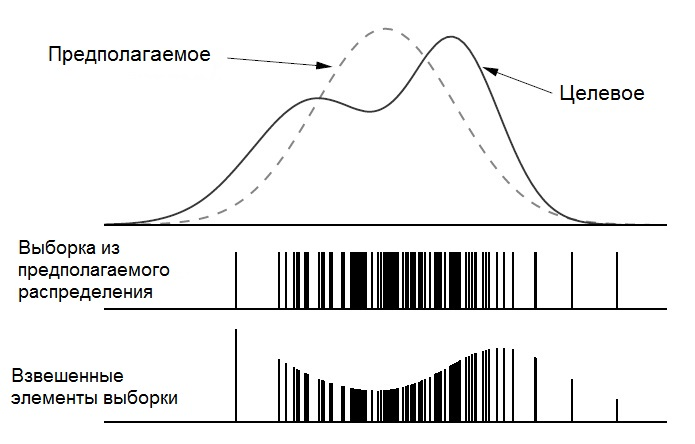
\includegraphics[width=0.8\linewidth]{135orig}}
	\caption{ ( Рис. 13.5 Элементы почти невозможно извлекать напрямую из искомого распределения (показано сплошной линией). Вместо этого функция выборки извлекает образцы выборки из предполагаемого распределения (пунктирная линия), что значительно проще. В нижней части рисунка извлекаются образцы из предполагаемого распределения согласно их весам значимости.) }
	\label{fig:135orig}
\end{figure}

Для определения фактора значимости будет полезно вычислить текущее предполагаемое распределение частиц пути во временном наборе. Допустив, что этот набор переменных пути из частиц $Y_{t-1}$ распределён в соответствии с $p(x_{1:t-1} | z_{1:t-1}, u_{1:t-1}, c_{1:t-1})$ (что является асимптотически верной аппроксимацией), частицы пути во временном наборе распределены согласно:\\

(13.19)
$$p(x_{1:t}^{[k]}|z_{1:t-1},u_{1:t},c_{1:t-1})=p(x_t^{[k]}|x_{t-1}^{[k]},u_t)p(x_{1:t-1}^{[k]}|z_{1:t-1},u_{1:t-1},c_{1:t-1})$$

Множитель $p(x_t^{[k]}|x_{t-1}^{[k]},u_t)$ показывает распределение выборки из выражения (13.12).

Целевое распределение принимает в расчёт распределение в момент времени $z_t$, а также соответствие $c_t$:\\

(13.20)
$$p(x_{1:t}^{[k]}|z_{1:t},u_{1:t},c_{1:t})$$

Процесс перевыборки принимает в расчёт разницу целевого и предполагаемого распределений.   Как обычно,  фактор значимости для перевыборки задан коэффициентами целевого и предполагаемого распределения:\\

(13.21)
\begin{equation*}
\begin{split}
w_t^{[k]}&=\frac{\text{целевое распределение }}{\text{предполагаемое распределение}}\\
&=\frac{p(x_{1:t}^{[k]}|z_{1:t},u_{1:t},c_{1:t})}{p(x_{1:t}^{[k]}|z_{1:t-1},u_{1:t},c_{1:t-1})}\\
&=\eta\,p(z_t|x_t^{[k]},c_t)
\end{split}
\end{equation*}

Последнее преобразование является прямым следствием следующего преобразования перечисления в (13.21):\\

(13.22)
\begin{equation*}
\begin{split}
p(&x_{1:t}^{[k]}|z_{1:t},u_{1:t},c_{1:t})\\
&=\eta\,p(z_t|x_{1:t}^{[k]},z_{1:t-1},u_{1:t},c_{1:t})p(x_{1:t}^{[k]}|z_{1:t-1},u_{1:t},c_{1:t})\\
&=\eta\,p(z_t|x_t^{[k]},c_t)p(x_{1:t}^{[k]}|z_{1:t-1},u_{1:t},c_{1:t-1})
\end{split}
\end{equation*}

Для вычисления вероятности $p(z_t|x_t^{[k]},c_t)$ в (13.21) будет необходимо выполнить дальнейшие преобразования. В частности, эта вероятность эквивалентна следующему интегрированию, где мы снова удаляем переменные, иррелевантные для прогноза измерения датчика:\\

(13.23)
\begin{equation*}
\begin{split}
w_t^{[k]}&=\eta\,\int p(z_t|m_{c_t},x_t^{[k]},c_t)p(m_{c_t}|x_t^{[k]},c_t)dm_{c_t}\\
&=\eta\,\int p(z_t|m_{c_t},x_t^{[k]},c_t)\underbrace{p(m_{c_t}|x_{1:t-1}^{[k]},z_{1:t-1},c_{1:t-1})}_{\sim\mathcal{N}(\mu_{c_t,t-1}^{[k]},\varSigma_{c_t,t-1}^{[k]})}dm_{c_t}
\end{split}
\end{equation*}

Здесь $\mathcal{N}(x;\mu,\varSigma)$ обозначает гауссово распределение по переменной $x$ с математическим ожиданием $\mu$ и ковариацией $\varSigma$.

Интеграция в (13.23) включает оценку местоположения наблюдаемого признака в момент времени $t$ и модель измерения. Для вычисления (13.23) в закрытом виде в FastSLAM выполняется та же самая линейная аппроксимация, используемая обновлении измерения на шаге 2. В частности, фактор значимости задан как\\

(13.24)
$$w_t^{[k]}\approx\eta\,|2\pi Q_t^{[k]}|^{-\frac{1}{2}}\exp\{-\frac{1}{2}(z_t-\hat{z}_t^{[k]})Q_t^{[k]-1}(z_t-\hat{z}_t^{[k]})\}$$

с ковариацией\\

(13.25)
$$Q_t^{[k]}=H_t^{[k]T}\varSigma_{n,t-1}^{[k]}H_t^{[k]}+Q_t$$

\begin{figure}[H]
	\center{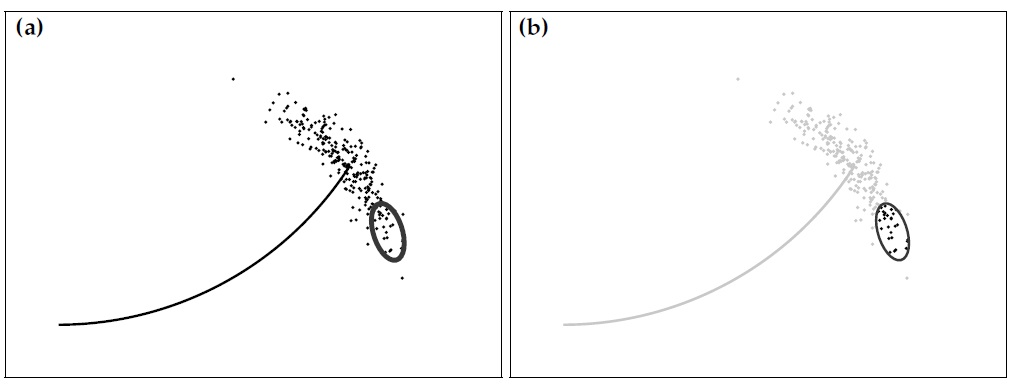
\includegraphics[width=1\linewidth]{136orig}}
	\caption{ ( Рис. 13.6 Несовпадение между предполагаемым и апостериорным распределением: показаны элементы прямой выборки в FastSLAM 1.0, и апостериорное распределение измерения (эллипс)(a). На Рис. (b) показан набор выборки после шага перевыборки.) }
	\label{fig:136orig}
\end{figure}

Это выражение является вероятностью текущего измерения $z_t$ при гауссовом распределении. Оно является результатом свёртки распределений (13.23), используя линейную аппроксимацию по $h$. Результирующие веса значимости используются для извлечения $M$ новых значений в временный набор значений выборки. С помощью этого процесса частицы сохраняются в пропорции их вероятности измерения.\\

Вместе эти три шага образуют правила обновления алгоритма FastSLAM 1.0 для задач SLAM с известной ассоциацией данных. Заметим, что время выполнения обновления не зависит от общей длины пути по времени $t$.
Фактически, в процессе генерации частицы в момент времени $t$ используется только последнее положение $x_{t-1}^{[k]}$.  Следовательно, прошлые положения могут отбрасываться. Это имеет полезное следствие, что ни требования вычислительного времени, ни занимаемой памяти FastSLAM не зависят от общего количества тактов времени, затраченных на получение данных.

Выводы по алгоритму FastSLAM 1.0 с известной ассоциацией данных приводятся в Таблице 13.1. Для простоты, эта реализация допускает что только один признак измеряется в один момент времени. Этот алгоритм упрощенно реализует разные шаги обновления. Сама реализация достаточно прямолинейна, ведь FastSLAM 1.0 является одним из простейших для реализации алгоритмов SLAM!

\begin{table}[H]
\begin{center}
\begin{tabular}{|l|}
\hline
{}\\
1:\textbf{ Algorithm FastSLAM 1.0\_known\_correspondence}$(z_t,c_t,u_t,Y_{t-1}):$\\
2:\hspace{5mm}$\textit{for}\,k=1\,\textit{to}\,M\,\textit{do}\qquad\qquad\qquad\qquad\qquad\qquad//\textit{цикл по всем частицам}$\\
3:\hspace{10mm}$\textit{получить}\langle x_{t-1}^{[k]},\langle\mu_{1,t-1}^{[k]},\varSigma_{1,t-1}^{[k]}\rangle,...,\langle\mu_{N,t-1}^{[k]},\varSigma_{N,t-1}^{[k]}\rangle\rangle\,\textit{из}\,Y_{t-1}$\\
4:\hspace{10mm}$x_t^{[k]}\sim p(x_t|x_{t-1}^{[k]},u_t)\qquad\qquad\quad\qquad\qquad//\textit{элемента положения}$\\
5:\hspace{10mm}$j=c_t\qquad\qquad\qquad\qquad\quad\qquad \qquad\qquad//\textit{наблюдаемый ориентир}$\\
6:\hspace{10mm}$\textit{если признак j ранее не наблюдался}$\\
7:\hspace{13mm}$\mu_{j,t}^{[k]}=h^{-1}(z_t,x_t^{[k]})\,\,\qquad\qquad\qquad\qquad//\textit{инициализировать среднее}$\\
8:\hspace{13mm}$H=h'(x_t^{[k]},\mu_{j,t}^{[k]})\qquad\qquad\qquad\qquad\quad//\textit{вычислить якобиан}$\\
9:\hspace{13mm}$\varSigma_{j,t}^{[k]}=H^{-1}Q_t(H^{-1})^T\,\,\,\,\qquad\qquad\qquad//\textit{инициализировать ковариацию}$\\
10:\hspace{12mm}$w^{[k]}=p_0\,\,\,\,\,\,\qquad\qquad\quad\qquad\qquad\qquad//\textit{веса знаимости по умолчанию}$\\
11:\hspace{9mm}$\textit{else}$\\
12:\hspace{13mm}$\hat{z}=h(\mu_{j,t-1}^{[k]},x_t^{[k]})\qquad\qquad\qquad\qquad//\textit{прогноз измерения}$\\
13:\hspace{12mm}
$H=h'(x_t^{[k]},\mu_{j,t-1}^{[k]})\,\qquad\qquad\qquad\quad//\textit{вычислить якобиан}$\\
14:\hspace{12mm}
$Q=H\varSigma_{j,t-1}^{[k]}H^T+Q_t\qquad\qquad\qquad//\textit{ковариация измерения}$\\
15:\hspace{12mm}
$K=\varSigma_{j,t-1}^{[k]}H^TQ^{-1}\,\,\quad\qquad\qquad\qquad//\textit{вычислить калмановское усиление}$\\
16:\hspace{12mm}
$\mu_{j,t}^{[k]}=\mu_{j,t-1}^{[k]}+K(z_t-\hat{z})\,\,\,\,\qquad\qquad//\textit{обновить среднее}$\\
17:\hspace{12mm}
$\varSigma_{j,t}^{[k]}=(I-K\,H)\varSigma_{j,t-1}^{[k]}\,\,\quad\qquad\qquad//\textit{обновить ковариацию}$\\
18:\hspace{12mm}
$w^{[k]}=|2\pi Q|^{-\frac{1}{2}}\exp\{-\frac{1}{2}(z_t-\hat{z}_n)^T$\\
\hspace{50mm}$Q^{-1}(z_t-\hat{z}_n)\}\,\,//\textit{фактор значимости}$\\
19:\hspace{9mm}$\textit{endif}$\\
20:\hspace{9mm}$\textit{для всех других признаков}\,j'\neq j\,\textit{do}\qquad\qquad//\textit{ненаблюдаемых признаков}$\\
21:\hspace{12mm}
$\mu_{j',t}^{[k]}=\mu_{j',t-1}^{[k]}\,\,\,\qquad\qquad\qquad\quad\qquad//\textit{оставить неизвменным}$\\
22:\hspace{12mm}
$\varSigma_{j',t}^{[k]}=\varSigma_{j',t-1}^{[k]}$\\
23:\hspace{9mm}$\textit{endfor}$\\
24:\hspace{4mm}$\textit{endfor}$\\
25:\hspace{4mm}$Y_t=\emptyset\,\,\,\qquad\qquad\qquad\quad\qquad\qquad\qquad\qquad//\textit{инициализировать новый набор частиц}$\\
26:\hspace{4mm}$\textit{повторить M раз}\emptyset\,\,\,\,\,\qquad\qquad\qquad\qquad\qquad\qquad//\textit{перевыборка M частиц }$\\
27:\hspace{9mm}$\textit{извлечь случайное k с вероятностью }\,\propto\,w^{[k]}\,//\textit{перевыборка}$\\
28:\hspace{9mm}$\textit{добавить }\langle x_t^{[k]},\langle\mu_{1,t}^{[k]},\varSigma_{1,t}^{[k]}\rangle,...,\langle\mu_N^{[k]},\varSigma_N^{[k]}\rangle\rangle\,\textit{ к }\,Y_t$\\
29:\hspace{4mm}$\textit{endfor}$\\
30:\hspace{4mm}$\textit{return}\,\,Y_t$\\
{}\\
\hline
\end{tabular}
\caption{(Таблица 13.1    FastSLAM 1.0 с известным соответствием.)}
\end{center}
\end{table}

\textbf{13.4	Улучшение предполагаемого распределения}\\

FASTSLAM 2.0

\textit{FastSLAM 2.0,} по большей части, эквивалентен FastSLAM 1.0, с одним важным исключением: в его предполагаемом распределении принимается во внимание $z_t$ при выполнении выборки по положению $x_t$.  Таким образом можно обойти ключевое ограничение FastSLAM 1.0.

На первый взгляд, разница невелика: читатель может припомнить, что FastSLAM 1.0 выполняет выборку положений только на основании сигналов управления $u_t$, а затем использует измерение $z_t$ для вычисления весов значимости. Это проблематично, когда точность сигналов управления относительно низка по сравнению с точностью датчиков робота. Такая ситуация показана на Рис. 13.6. Предположение генерируется на основании большого спектра элементов выборки, показанных на Рис. 13.6a, но только малое подмножество этих элементов имеет высокое правдоподобие, как показано в виде эллипсоида. После перевыборки только частицы внутри эллипсоида сохранятся с относительно высоким правдоподобием. FastSLAM 2.0 обходит эту проблему выполнением выборки из положений на основе измерения $z_t$ вдобавок к сигналу управления $u_t$. Таким образом, FastSLAM 2.0 более эффективен по сравнению с FastSLAM 1.0. С другой стороны, FastSLAM 2.0 более сложен в реализации по сравнению с FastSLAM 1.0, и математический вывод также более труден.\\

\textbf{13.4.1	Обобщение апостериорной вероятности пути выборкой нового положения}\\

В FastSLAM 2.0 положение $x_t^{[k]}$ извлекается из апостериорного распределения\\

(13.26)
$$x_t^{[k]}\sim p(x_t|x_{1:t-1}^{[k]},u_{1:t},z_{1:t},c_{1:t})$$

Это распределение отличается от предполагаемого распределения, представленного в (13.12) в котором (13.26) принимает измерение $z_t$ в расчёт, вместе с соответствием $c_t$. В частности, выражение в (13.26) зависит от $z_{1:t}$, а алгоритм выборки положения FastSLAM 1.0 зависит от $z_{1:t-1}$.

К сожалению, это требует и более сложной математики. В частности, механизм выполнения выборки из (13.26) требует дальнейшего анализа. Во-первых, перепишем (13.26) в терминах «известных» распределений, таких, как модели измерения и движения, и гауссова оценка признака в $k$-й частице.\\

(13.27)
\begin{equation*}
\begin{split}
p(&x_t|x_{1:t-1}^{[k]},u_{1:t},z_{1:t},c_{1:t})\\
&\overset{\text{Bayes}}{=}\frac{p(z_t|x_t,x_{1:t-1}^{[k]},u_{1:t},z_{1:t-1},c_{1:t})p(x_t|x_{1:t-1}^{[k]},u_{1:t},z_{1:t-1},c_{1:t})}{p(z_t|x_{1:t-1}^{[k]},u_{1:t},z_{1:t-1},c_{1:t})}\\
&\quad=\eta^{[k]}p(z_t|x_t,x_{1:t-1}^{[k]},u_{1:t},z_{1:t-1},c_{1:t})p(x_t|x_{1:t-1}^{[k]},u_{1:t},z_{1:t-1},c_{1:t})\\
&\overset{\text{Markov}}{=}\eta^{[k]}p(z_t|x_t,x_{1:t-1}^{[k]},u_{1:t},z_{1:t-1},c_{1:t});p(x_t|x_{t-1}^{[k]},u_t)\\
&\quad=\eta^{[k]}\int p(z_t|m_{c_t},x_t,x_{1:t-1}^{[k]},u_{1:t},z_{1:t-1},c_{1:t})\\
&\qquad\qquad p(m_{c_t}|x_t,x_{1:t-1}^{[k]},u_{1:t},z_{1:t-1},c_{1:t})dm_{c_t}p(x_t|x_{t-1}^{[k]},u_t)\\
&\overset{\text{Markov}}{=}\eta^{[k]}\int\underbrace{p(z_t|m_{c_t},x_t,c_t)}_{\sim\mathcal{N}(z_t;h(m_{c_t},x_t),Q_t)}\underbrace{p(m_{c_t}|x_{1:t-1}^{[k]},z_{1:t-1},c_{1:t-1})}_{\sim\mathcal{N}(m_{c_t};\mu_{c_t,t-1}^{[k]},\varSigma_{c_t,t-1}^{[k]})}dm_{c_t}\\
&\hspace{50mm}\underbrace{p(x_t|x_{t-1}^{[k]},u_t)}_{\sim\mathcal{N}(x_t;g(x_{t-1}^{[k]},u_t),R_t)}
\end{split}
\end{equation*}

Это выражение показывает, что наше распределение извлечения выборки действительно является свёрткой двух гауссианов, перемноженных на третий. В общем случае SLAM распределение по выборке не имеет закрытого вида, из которого можно легко извлекать элементы выборки. Виной всему функция $h$: если бы она была линейна, вероятность была бы гауссовой, что станет понятным чуть ниже. Фактически, даже интеграл в (13.27) не имеет решения в закрытом виде, поэтому выборка из вероятности (13.27) затруднена.

Это наблюдение побуждает заменить $h$ линейной аппроксимацией. Как часто встречается в книге, это приближение получается с помощью разложения в ряд Тейлора первого порядка, заданного следующей линейной функцией:\\

(13.28)
$$h(m_{c_t},x_t)\approx\hat{z}_t^{[k]}+H_m(m_{c_t}-\mu_{c_t,t-1}^{[k]})+H_x(x_t-\hat{x}_t^{[k]})$$

Здесь используем следующие сокращения:\\

(13.29)
$$\hat{z}_t^{[k]}=h(\mu_{c_t,t-1}^{[k]},\hat{x}_t^{[k]})$$

(13.30)
$$\hat{x}_t^{[k]}=g(x_{t-1}^{[k]},u_t)$$

Матрицы $H_m$ и $H_x$ являются якобианами $h$. Они также производные $h$ по отношению к $m_{c_t}$ и $x_t$, соответственно, вычисленные по ожидаемым значениям аргументов:\\

(13.31)
$$H_m=\nabla_{m_{c_t}}h(m_{c_t},x_t)|_{x_t=\hat{x}_t^{[k]};m_{c_t}=\mu_{c_t,t-1}^{[k]}}$$

(13.32)
$$H_x=\nabla_{x_t}h(m_{c_t},x_t)|_{x_t=\hat{x}_t^{[k]};m_{c_t}=\mu_{c_t,t-1}^{[k]}}$$

С этой аппроксимацией искомое распределение выборки (13.27) является гауссианом со следующими параметрами:\\

(13.33)
$$\varSigma_{x_t}^{[k]}=[H_x^TQ_t^{[k]-1}H_x+R_t^{-1}]^{-1}$$

(13.34)
$$\mu_{x_t}^{[k]}=\varSigma_{x_t}^{[k]}H_x^TQ_t^{[k]-1}(z_t-\hat{z}_t^{[k]})+\hat{x}_t^{[k]}$$

где матрица $Q_t^{[k]}$ определена следующим образом:\\

(13.35)
$$Q_t^{[k]}=Q_t+H_m\varSigma_{c_t,t-1}^{[k]}H_m^T$$

Заметим, что для линейной аппроксимации теорема о свёртке имеет закрытый вид для интегрального члена в (13.27):\\

(13.36)
$$\mathcal{N}(z_t;\hat{z}_t^{[k]}+H_xx_t-H_x\hat{x}_t^{[k]},Q_t^{[k]})$$

Распределение выборки (13.27) сейчас задано в виде произведения этого нормального распределения и самого правого члена в (13.27), нормального  $\mathcal{N}(x_t;\hat{x}_t^{[k]},R_t)$. Записав в гауссовой форме, получим\\

(13.37)
$$p(x_t|x_{1:t-1}^{[k]},u_{1:t},z_{1:t},c_{1:t})=\eta\,\exp\{-P_t^{[k]}\}$$

с\\

(13.38)
\begin{equation*}
\begin{split}
P_t^{[k]}=\frac{1}{2}&[(z_t-\hat{z}_t^{[k]}-H_xx_t+H_x\hat{x}_t^{[k]})^TQ_t^{[k]-1}(z_t-\hat{z}_t^{[k]}-H_xx_t+H_x\hat{x}_t^{[k]})\\
&+(x_t-\hat{x}_t^{[k]})^TR_t^{-1}(x_t-\hat{x}_t^{[k]})]
\end{split}
\end{equation*}

Очевидно, это выражение квадратично по целевой переменной $x_t$, поэтому $p(x_t|x_{1:t-1}^{[k]},u_{1:t},z_{1:t},c_{1:t})$ является гауссианом.  Математическое ожидание и ковариация этого гауссиана
эквивалентны минимуму $P_t^{[k]}$ и кривизны. Они идентичны
вычислению первой и второй производной $P_t^{[k]}$ по $x_t$:

(13.39)
\begin{equation*}
\begin{split}
\frac{\partial P_t^{[k]}}{\partial x_t}&=-H_x^TQ_t^{[k]-1}(z_t-\hat{z}_t^{[k]}-H_xx_t+H_x\hat{x}_t^{[k]})+R_t^{-1}(x_t-\hat{x}_t^{[k]})\\
&=(H_x^TQ_t^{[k]-1}H_x+R_t^{-1})x_t-H_x^TQ_t^{[k]-1}(z_t-\hat{z}_t^{[k]}+H_x\hat{x}_t^{[k]})-R_t^{-1}\hat{x}_t^{[k]}
\end{split}
\end{equation*}

(13.40)
\begin{equation*}
\begin{split}
\frac{\partial^2 P_t^{[k]}}{\partial x_t^2}=H_x^TQ_t^{[k]-1}H_x+R_t^{-1}
\end{split}
\end{equation*}

Ковариация $\varSigma_{x_t}^{[k]}$ распределения выборки получается обращением второй производной\\

(13.41)
$$\varSigma_{x_t}^{[k]}=[H_x^TQ_t^{[k]-1}H_x+R_t^{-1}]^{-1}$$

Математическое ожидание $\mu_{x_t}^{[k]}$ распределения выборки получается установкой первой производной в (13.39) в нуль. Это даст:\\

(13.42)
\begin{equation*}
\begin{split}
\mu_{x_t}^{[k]}&=\varSigma_{x_t}^{[k]}[H_x^TQ_t^{[k]-1}(z_t-\hat{z}_t^{[k]}+H_x\hat{x}_t^{[k]})+R_t^{-1}\hat{x}_t^{[k]}]\\
&=\varSigma_{x_t}^{[k]}H_x^TQ_t^{[k]-1}(z_t-\hat{z}_t^{[k]})+\varSigma_{x_t}^{[k]}[H_x^TQ_t^{[k]-1}H_x+R^{-1}]\hat{x}_t^{[k]}\\
&=\varSigma_{x_t}^{[k]}H_x^TQ_t^{[k]-1}(z_t-\hat{z}_t^{[k]})+\hat{x}_t^{[k]}
\end{split}
\end{equation*}

Этот гауссиан является аппроксимацией искомого распределения выборки (13.26) в FastSLAM 2.0.  Очевидно, это предполагаемое распределение значительно сложнее, чем используемое для FastSLAM 1.0 в выражении (13.12).\\

\textbf{13.4.2	Обновление оценки наблюдаемого признака}\\

Так же, как и первая версия алгоритма FastSLAM, FastSLAM 2.0  выполняет обновление апостериорной вероятности по оценкам признака на основе измерения $z_t$ и выборки по положению $x_t^{[k]}$. Оценки в момент времени $t-1$ снова выражены в виде
математического ожидания $\mu_{j,t-1}^{[k]}$ и ковариации $\varSigma_{j,t-1}^{[k]}$. Обновлённые оценки обозначены $\mu_{j,t}^{[k]}$ и $\varSigma_{j,t}^{[k]}$. Последовательность обновления зависит от того, наблюдался или нет признак $j$ в момент времени $t$. Для $j\neq c_t$ уже было определено выражение (13.4) и установлено, что апостериорное распределение остаётся неизменным. Это означает, что, вместо обновления оценки, ее можно просто скопировать.

Для наблюдаемого признака $j=c_t$ ситуация более сложная. В выражении (13.5) уже установлено апостериорное распределение по наблюдаемому признаку. Повторим его с индексом частицы $k$:\\

(13.43)
\begin{equation*}
\begin{split}
p(&m_{c_t}|x_t^{[k]},c_{1:t},z_{1:t})\\
&=\eta\,\underbrace{p(z_t|m_{c_t},x_t^{[k]},c_t)}_{\sim\mathcal{N}(z_t;h(m_{c_t},x_t^{[k]}),Q_t)}\underbrace{p(m_{c_t}|x_{1:t-1}^{[k]},z_{1:t-1},c_{1:t-1})}_{\sim\mathcal{N}(m_{c_t};\mu_{c_t,t-1}^{[k]},\varSigma_{c_t,t-1}^{[k]})}
\end{split}
\end{equation*}

Так же как в выражении (13.27) нелинейность $h$ не позволяет выразить апостериорную вероятность в виде гауссиана, что противоречит выражению для оценки признаков FastSLAM 2.0 в виде гауссовой функции. К счастью, решение лежит в той же самой линеаризации, которая уже обсуждалась выше:\\

(13.44)
$$h(m_{c_t},x_t)\approx\hat{z}_t^{[k]}+H_m(m_{c_t}-\mu_{c_t,t-1}^{[k]})$$

Заметим, что $x_t$ не является свободной переменной, поэтому третий член в выражении (13.28) можно отбросить. Эта аппроксимация даст вероятность вида (13.43). Гауссиан в целевой переменной $m_{c_t}$:\\

(13.45)
\begin{equation*}
\begin{split}
p(&m_{c_t}|x_t^{[k]},c_{1:t},z_{1:t})\\
&=\eta\,\exp\,\{-\frac{1}{2}(z_t-\hat{z}_t^{[k]}-H_m(m_{c_t}-\mu_{c_t,t-1}^{[k]}))Q_t^{-1}\\
&\qquad\qquad(z_t-\hat{z}_t^{[k]}-H_m(m_{c_t}-\mu_{c_t,t-1}^{[k]}))\\
&\qquad\qquad-\frac{1}{2}(m_{c_t}-\mu_{c_t,t-1}^{[k]})\varSigma_{c_t,t-1}^{[k]-1}(m_{c_t}-\mu_{c_t,t-1}^{[k]})\}
\end{split}
\end{equation*}

Новые математическое ожидание и ковариация получаются, используя стандартные уравнения обновления измерения EKF:\\

(13.46)
$$K_t^{[k]}=\varSigma_{c_t,t-1}^{[k]}H_m^TQ_t^{[k]-1}$$

(13.47)
$$\mu_{c_t,t}^{[k]}=\mu_{c_t,t-1}^{[k]}+K_t^{[k]}(z_t-\hat{z}_t^{[k]})$$

(13.48)
$$\varSigma_{c_t,t}^{[k]}=(I-K_t^{[k]}H_m)\varSigma_{c_t,t-1}^{[k]}$$

Заметим, что это несколько сложнее, чем обновление в FastSLAM 1.0, но дополнительные усилия в реализации часто окупаются за счет улучшенной точности.\\

\textbf{13.4.3	Вычисление факторов значимости}\\

Пока что сгенерированные частицы не совпадают с искомой апостериорной вероятностью. В FastSLAM 2.0 это вызвано нормализующим членом $\eta^{[k]}$ в (13.27), который обычно различен для каждой частицы $k$. Эти различия еще е учтены в процессе перевыборки. Также как в FastSLAM 1.0, фактор значимости выражен следующим коэффициентом.\\

(13.49)
$$w_t^{[k]}=\frac{\text{target distribution}}{\text{proposal distribution}}$$

И снова, целевое распределение, которое бы хотелось выразить с помощью частиц, задано апостериорной вероятностью по пути  $p(x_t^{[k]}|z_{1:t}, u_{1:t}, c_{1:t})$.  Используя асимптотически корректные допущения, что пути $x_{1:t-1}^{[k]}$ были сгенерированы согласно целевому распределению, взятому на шаг ранее, $p(x_{1:t-1}^{[k]}|z_{1:t-1}, u_{1:t-1}, c_{1:t-1})$,
заметим, что предполагаемое распределение теперь задано произведением \\

(13.50)
$$p(x_{1:t-1}^{[k]}|z_{1:t-1}, u_{1:t-1}, c_{1:t-1})\,p(x_t^{[k]}|x_{1:t-1}^{[k]},u_{1:t}, z_{1:t}, c_{1:t})$$

второй член произведения является распределением выборки положения (13.27). Вес значимости получается следующим образом:\\

(13.51)
\begin{equation*}
\begin{split}
w_t^{[k]}&=\frac{p(x_t^{[k]}|u_{1:t}, z_{1:t}, c_{1:t})}{p(x_t^{[k]}|x_{1:t-1}^{[k]},u_{1:t}, z_{1:t}, c_{1:t})p(x_{1:t-1}^{[k]}|u_{1:t-1},z_{1:t-1},c_{1:t-1})}\\
&=\frac{p(x_t^{[k]}|x_{1:t-1}^{[k]},u_{1:t}, z_{1:t}, c_{1:t})p(x_{1:t-1}^{[k]}|u_{1:t},z_{1:t},c_{1:t})}{p(x_t^{[k]}|x_{1:t-1}^{[k]},u_{1:t}, z_{1:t}, c_{1:t})p(x_{1:t-1}^{[k]}|u_{1:t-1},z_{1:t-1},c_{1:t-1})}\\
&=\frac{p(x_{1:t-1}^{[k]}|u_{1:t},z_{1:t},c_{1:t})}{p(x_{1:t-1}^{[k]}|u_{1:t-1},z_{1:t-1},c_{1:t-1})}\\
&\overset{\text{Bayes}}{=}\,\eta\,\frac{p(z_t|x_{1:t-1}^{[k]},u_{1:t}, z_{1:t-1}, c_{1:t})p(x_{1:t-1}^{[k]}|u_{1:t},z_{1:t-1},c_{1:t})}{p(x_{1:t-1}^{[k]}|u_{1:t-1},z_{1:t-1},c_{1:t-1})}\\
&\overset{\text{Markov}}{=}\,\eta\,\frac{p(z_t|x_{1:t-1}^{[k]},u_{1:t}, z_{1:t-1}, c_{1:t})p(x_{1:t-1}^{[k]}|u_{1:t-1},z_{1:t-1},c_{1:t-1})}{p(x_{1:t-1}^{[k]}|u_{1:t-1},z_{1:t-1},c_{1:t-1})}\\
&=\eta\,p(z_t|x_{1:t-1}^{[k]},u_{1:t}, z_{1:t-1}, c_{1:t})
\end{split}
\end{equation*}

Читатель может заметить, что это выражение является инверсией нормировочной постоянной $\eta^{[k]}$ в (13.27). Дальнейшие преобразования ведут к следующему виду:\\

(13.52)
\begin{equation*}
\begin{split}
w_t^{[k]}&=\eta\int p(z_t|x_t,x_{1:t-1}^{[k]},u_{1:t},z_{1:t-1},c_{1:t})\\
&\qquad\qquad p(x_t|x_{1:t-1}^{[k]},u_{1:t},z_{1:t-1},c_{1:t})dx_t\\
&\overset{\text{Markov}}{=}\,\eta\int p(z_t|x_t,x_{1:t-1}^{[k]},u_{1:t},z_{1:t-1},c_{1:t})p(x_t|x_{t-1}^{[k]},u_t)dx_t\\
&=\eta\int\int p(z_t|m_{c_t},x_t,x_{1:t-1}^{[k]},u_{1:t},z_{1:t-1},c_{1:t})\\
&\qquad\qquad p(m_{c_t}|x_t,x_{1:t-1}^{[k]},u_{1:t},z_{1:t-1},c_{1:t})dm_{c_t}p(x_t|x_{t-1}^{[k]},u_t)dx_t\\
&\overset{\text{Markov}}{=}\,\eta\int\underbrace{p(x_t|x_{t-1}^{[k]},u_t)}_{\sim\mathcal{N}(x_t;g(\hat{x}_{t-1}^{[k]},u_t),R_t)}\int\underbrace{p(z_t|m_{c_t},x_t,c_t)}_{\sim\mathcal{N}(z_t;h(m_{c_t},x_t),Q_t)}\\
&\qquad\qquad\underbrace{p(m_{c_t}|x_{1:t-1}^{[k]},u_{1:t-1},z_{1:t-1},c_{1:t-1})}_{\sim\mathcal{N}(m_{c_t};\mu_{c_t,t-1}^{[k]},\varSigma_{c_t,t-1}^{[k]})}dm_{c_t}dx_t
\end{split}
\end{equation*}

Мы обнаружили, что это выражение снова можно аппроксимировать гауссовой функцией по измерениям $z_t$ путём линеаризации функции $h$. Как легко показать, математическое ожидание результирующего гауссиана $\hat{z}_t$, и его ковариация равны\\

(13.53)
$$L_t^{[t]}=H_x^TQ_tH_x+H_m\varSigma_{c_t,t-1}^{[k]}H_m^T+R_t$$

другими словами, не нормализованный множитель значимости $k$-й частицы задан следующим выражением:\\

(13.54)
$$w_t^{[k]}=|2\pi L_t^{[t]}|^{-\frac{1}{2}}\exp\{-\frac{1}{2}(z_t-\hat{z}_t)L_t^{[t]-1}(z_t-\hat{z}_t)\}$$

Так же, как FastSLAM 1.0, частицы, сгенерированные на этапах 1 и 2, вместе с фактором значимости, вычисленным на этапе 3, собираются во временный набор частиц.

Финальный шаг обновления FastSLAM 2.0 – перевыборка.  Так же, как в FastSLAM 1.0, FastSLAM 2.0 извлекает (с заменой) $M$ частиц  из временного набора частиц. Каждая частица извлекается с вероятностью, пропорциональной фактору значимости $w_t^{[k]}$. Результирующий набор частиц асимптотически выражает искомую факторизованную апостериорную вероятность $t$.

\begin{figure}[H]
	\center{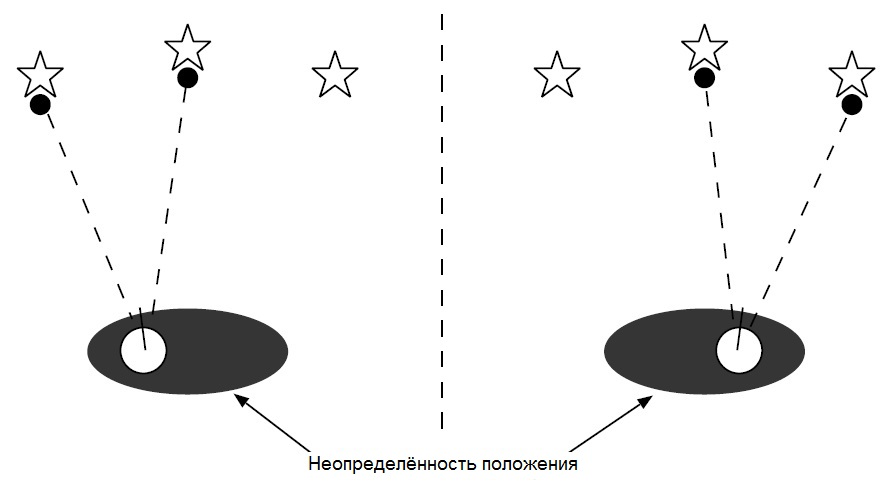
\includegraphics[width=0.8\linewidth]{137orig}}
	\caption{ ( Рис. 13.7 Проблема ассоциации данных в SLAM. На рисунке показано, что лучшая ассоциация данных может быть различной даже внутри областей с высоким правдоподобием положения робота.) }
	\label{fig:137orig}
\end{figure}

\textbf{13.5	Неизвестная ассоциация данных}\\

Этот раздел обобщает обе переменные алгоритма FastSLAM для случая, когда переменные соответствия $c_{1:t}$ неизвестны. Ключевым преимуществом использования многочастичных фильтров для SLAM являются отдельные для каждой частицы локальные решения ассоциации данных.

Напоминаем читателю, что задача ассоциации данных в момент времени $t$ является задачей определения переменной $c_t$ на основе доступных данных. Эта проблема показана на Рис. 13.7. Здесь робот наблюдает два признака окружающей среды. В зависимости от относительного положения робота и измерения этих признаков, эти измерения соответствуют различным признакам карты (показаны звёздочками на Рис. 13.7).

Пока что обсуждались различные методы ассоциации данных, используя ряд таких методов, как максимум правдоподобия. эти методы объединяет то, что для всего фильтра имеется только одна ассоциация данных на измерение. FastSLAM, из-за использования нескольких частиц, способен определить соответствие для каждой частицы. Таким образом, фильтр не только выполняет выборку по траекториям робота, но также по возможным решениям ассоциации данных на этом пути. 

Это является одним из ключевых свойств FastSLAM, отделяющим его от большого семейства алгоритмов SLAM. Пока малое подмножество частиц основано на верной ассоциации данных, ошибки ассоциации данных фатальными не являются, как в случае методов EKF. Частицы, подверженные таким ошибкам, могут создавать противоречивые карты, которые увеличивают вероятность того, что они будут исключены при перевыборке из будущих карт.

Математическое определение ассоциации данных для каждой частицы очевидно, обобщая ассоциацию данных для каждого фильтра. Для каждой частицы сохраняется локальный набор переменных ассоциации данных, обозначаемых $\hat{c}_t^{[k]}$. При ассоциации данных методом максимального правдоподобия каждый $\hat{c}_t^{[k]}$ определяется
максимизацией правдоподобия измерения $z_t$:\\

(13.55)
$$\hat{c}_t^{[k]}=\underset{c_t}{\text{argmax}}\,p(z_t|c_t,\hat{c}_{1:t-1}^{[k]},x_{1:t}^{[k]},z_{1:t-1}u_{1:t})$$

Альтернативой является алгоритм выборки ассоциации данных (data association sampler- DAS), выполняющий выборку переменной ассоциации данных в соответствии с правдоподобием\\

(13.56)
$$\hat{c}_t\sim\eta\,p(z_t|c_t,\hat{c}_{1:t-1},x_{1:t}^{[k]},z_{1:t-1}u_{1:t})$$

Оба метода, и метод максимального правдоподобия, и DAS, позволяют оценить количество признаков на карте. Методы SLAM на основе методов максимального правдоподобия, создают новые признаки на карте, если правдоподобие падает ниже порога $p_0$ для всех известных признаков на карте. DAS выполняет стохастическую ассоциацию наблюдаемого измерения с новым, прежде ненаблюдаемым признаком. Это выполняется с вероятностью, пропорциональной $\eta p_0$, где $\eta$ является нормализующим членом, определенным в (13.56).\\

(13.57)
$$\hat{c}_t^{[k]}\sim\eta\,p(z_t|c_t,\hat{c}_{1:t-1}^{[k]},x_{1:t}^{[k]},z_{1:t-1}u_{1:t})$$

Для обоих методов, правдоподобие вычисляется следующим образом:\\

(13.58)
\begin{equation*}
\begin{split}
p(&z_t|c_t,\hat{c}_{1:t-1}^{[k]},x_{1:t}^{[k]},z_{1:t-1},u_{1:t})\\
&=\int p(z_t|m_{c_t},c_t,\hat{c}_{1:t-1}^{[k]},x_{1:t}^{[k]},z_{1:t-1},u_{1:t})\\
&\qquad\qquad p(m_{c_t}|c_t,\hat{c}_{1:t-1}^{[k]},x_{1:t}^{[k]},z_{1:t-1},u_{1:t})dm_{c_t}\\
&=\int\underbrace{p(z_t|m_{c_t},c_t,x_t^{[k]})}_{\sim\mathcal{N}(z_t;h(m_{c_t},x_t^{[k]}),Q_t)}\underbrace{p(m_{c_t}|\hat{c}_{1:t-1}^{[k]},x_{1:t-1}^{[k]},z_{1:t-1})}_{\sim\mathcal{N}(\mu_{c_t,t-1}^{[k]},\varSigma_{c_t,t-1}^{[k]})}dm_{c_t}
\end{split}
\end{equation*}

Линеаризация функции $h$ позволяет получить его в закрытом виде:\\

(13.59)
\begin{equation*}
\begin{split}
p(&z_t|c_t,\hat{c}_{1:t-1}^{[k]},x_t^{[k]},z_{1:t-1},u_{1:t})\\
&=|2\pi Q_t^{[k]}|^{-\frac{1}{2}}\exp\{-\frac{1}{2}(z_t-h(\mu_{c_t,t-1}^{[k]},x_t^{[k]}))^TQ_t^{[k]-1}(z_t-h(\mu_{c_t,t-1}^{[k]},x_t^{[k]}))\}
\end{split}
\end{equation*}

Переменная $Q_t^{[k]}$ была определена в выражении (13.35), как функция переменной ассоциации данных $c_t$. Новые признаки добавляются к карте как описано выше.  В методе ML новый признак добавляется, когда вероятность $p(z_t|c_t, \hat{c}_{1:t-1}^{[k]},x_t^{[k]},z_{1:t-1},u_{1:t})$ падает ниже порога$p_0$. DAS включает новую гипотезу, что наблюдение, соответствующее прежде ненаблюдаемое действие в набор гипотез, и выполняет выборку с вероятностью $\eta p_0$.\\

\textbf{13.6	Управление картой}\\

Управление картой FastSLAM, в основном, аналогично, EKF SLAM с небольшим количеством частиц, поскольку в FastSLAM ассоциация данных выполняется на уровне отдельных частиц.

Так же как в альтернативных алгоритмах SLAM, любой вновь добавленный признак требует инициализацию нового фильтра Калмана. Во многих задачах SLAM функция измерения $h$ \textit{обратима}. Это происходит, например, когда робот выполняет измерение расстояния и направления на признаки на плоскости, и единичного измерения достаточно для появления новой (невырожденной) оценки по местонахождению признака. Инициализация EKF очевидна:\\

(13.60)
$$x_t^{[k]}\sim p(x_t|x_{t-1}^{[k]},u_t)$$

(13.61)
$$\mu_{n,t}^{[k]}=h^{-1}(z_t,x_t^{[k]})$$

(13.62)
$$\varSigma_{n,t}^{[k]}=(H_{\hat{c}}^{[k]T}Q_t^{-1}H_{\hat{c}}^{[k]})^{-1}\qquad\text{где}\qquad H_{\hat{c}}^{[k]}=h'(\mu_{n,t}^{[k]},x_t^{[k]})$$

(13.63)
$$w_t^{[k]}=p_0$$

Заметим, что для вновь обнаруженных признаков выборка по положению $x_t^{[k]}$ выполняется в соответствии с моделью движения $p(x_t|x_{t-1}^{[k]}, u_t)$. Это распределение эквивалентно выборке из распределения FastSLAM (13.26) в ситуациях, когда отсутствуют предыдущие оценки для наблюдаемого признака.

Методы инициализации для ситуаций, когда $h$ необратимо, обсуждались в работах Динса и Хеберта (Deans and Hebert, 2002). В таких ситуациях требуется накопление нескольких измерений, чтобы получить хорошую оценку линеаризации $h$.

Чтобы обрабатывать ошибочно привнесённые на карту признаки, FastSLAM имеет механизм уничтожения признаков, которые не поддержаны достаточным объёмом наблюдений. Так же как в EKF SLAM, в FastSLAM это выполняется отслеживанием логарифма шансов существования отдельных признаков на карте.

В частности, при наблюдении признака его логарифм шансов на существование увеличивается на фиксированное значение, которое вычисляется по стандартной формуле теоремы Байеса. Похожим образом, когда признак не наблюдается в ситуации, когда он должен был присутствовать, такая отрицательная информация вызывает уменьшение переменной существования признака на фиксированное значение. Признаки, значение переменной существования которых падает ниже порогового значения, удаляются из списка частиц. Так же возможно реализовать временный список признаков в FastSLAM, что технически тривиально, поскольку для каждого признака имеется собственная частица.\\

\textbf{13.7	Алгоритмы FastSLAM} \\

В Таблицах 13.2 и 13.3 приводятся итоговые алгоритмы FastSLAM с неизвестной ассоциацией данных. В обоих алгоритмах частицы заданы в виде\\

(13.64)
$$Y_t^{[k]}=\langle x_t^{[k]},N_t^{[k]},\langle\mu_{1,t}^{[k]},\varSigma_{1,t}^{[k]},\tau_1^{[k]}\rangle,...,\langle\mu_{N_t^{[k]},t}^{[k]},\varSigma_{N_t^{[k]},t}^{[k]},\tau_{N_t^{[k]}}^{[k]}\rangle\rangle$$

Вдобавок к положению $x_t^{[k]}$ и оценкам признаков $\mu_{n,t}^{[k]}$  и $\varSigma_{n,t}^{[k]}$ в каждой частице сохраняется некоторое количество признаков $N_t^{[k]}$ на локальной карте, а каждый признак несёт вероятностную оценку существования $\tau_n^{[k]}$. Для выполнения итерации фильтра требуется время, линейно зависящее от максимального количества признаков $max_k N_t^{[k]}$ на каждой карте, и от числа частиц $M$. Ниже будет обсуждаться более совершенная структура данных, которая позволяет создавать более эффективные реализации.

Заметим, что обе версии FastSLAM, описанные здесь, основаны на одном измерении в один момент времени. Как и прежде, это допущение сделано для удобства записи, как было выполнено для многих методов SLAM, описанных в предыдущих главах.\\

\textbf{13.8	Эффективная реализация}\\

На первый взгляд, может показаться, что каждое обновление в FastSLAM требует времени $O(MN)$, где $M$ – число частиц, а $N$ –число признаков на карте. Линейная сложность по $M$ неизбежна, учитывая, что при каждом обновлении необходимо обработать $M$ частиц. Линейная сложность по $N$ является результатом выполнения перевыборки. Когда частица извлекается при перевыборке больше одного раза, наивная реализация может дублировать всю карту, связанную с частицей. Такой процесс дублирования линейно зависит от размера карты $N$. Более того, наивная реализация ассоциации данных может привести к оценке правдоподобности измерения для каждого из $N$ признаков на карте, что снова повлечёт линейную зависимость вычислительной сложности от $N$. Заметим, что плохая реализация процесса выборки может легко увеличить сложность обновления ещё на $\log N$.\\

\begin{table}[H]
\begin{center}
\begin{tabular}{|l|}
\hline
{}\\
1:\textbf{ Algorithm FastSLAM 1.0}$(z_t,u_t,Y_{t-1}):$\\
2:\hspace{5mm}$\textit{for}\,k=1\,\textit{to}\,M\,\textit{do}\qquad\qquad\qquad\qquad\qquad\qquad//\textit{цикл по всем частицам}$\\
3:\hspace{10mm}$\textit{retrieve}\langle x_{t-1}^{[k]},N_{t-1}^{[k]},\langle\mu_{1,t-1}^{[k]},\varSigma_{1,t-1}^{[k]},i_1^{[k]}\rangle,...,$\\
\hspace{30mm}$\langle\mu_{N_{t-1}^{[k]},t-1}^{[k]},\varSigma_{N_{t-1}^{[k]},t-1}^{[k]},i_{N_{t-1}^{[k]},t-1}^{[k]}\rangle\rangle\,\textit{из }\,Y_{t-1}$\\
4:\hspace{10mm}$x_t^{[k]}\sim p(x_t|x_{t-1}^{[k]},u_t)\qquad\qquad\quad\qquad\qquad//\textit{элемент положения}$\\
5:\hspace{10mm}$\textit{for}\,j=1\,\textit{to}\,N_{t-1}^{[k]}\,\textit{do}\,\,\qquad\qquad\qquad\qquad\quad//\textit{правдоподобия измерения}$\\
6:\hspace{13mm}$\hat{z}_j=h(\mu_{j,t-1}^{[k]},x_t^{[k]})\,\,\,\,\quad\quad\qquad\qquad\qquad//\textit{прогноз измерения}$\\
7:\hspace{12mm}
$H_j=h'(\mu_{j,t-1}^{[k]},x_t^{[k]})\,\,\,\,\,\qquad\qquad\qquad\quad//\textit{вычислить якобиан}$\\
8:\hspace{12mm}
$Q_j=H_j\varSigma_{j,t-1}^{[k]}H_j^T+Q_t\qquad\qquad\qquad//\textit{ковариация измерения}$\\
9:\hspace{12mm}
$w_j=|2\pi Q_j|^{-\frac{1}{2}}\exp\{-\frac{1}{2}(z_t-\hat{z}_j)^T$\\
\hspace{40mm}$Q_j^{-1}(z_t-\hat{z}_j)\}\,\,\quad\qquad//\textit{правдоподобие соответствия}$\\
10:\hspace{9mm}$\textit{endfor}$\\
11:\hspace{9mm}$w_{1+N_{t-1}^{[k]}}=p_0\qquad\qquad\qquad\qquad\quad\qquad//\textit{фактор значимости, новый признак}$\\
12:\hspace{9mm}$w^{[k]}=\max\, w_j\,\,\,\quad\qquad\qquad\qquad\quad\qquad//\textit{максимальное правдоподобие соответствия}$\\
13:\hspace{9mm}$\hat{c}=\text{argmax}\,w_j\,\,\,\qquad\qquad\quad\qquad\quad\qquad//\textit{индекс максимального правдоподобия признака}$\\
14:\hspace{9mm}$N_t^{[k]}=\max\{N_{t-1}^{[k]},\hat{c}\}\,\,\,\,\quad\quad\qquad\quad\qquad//\textit{новое число признаков на карте}$\\
15:\hspace{9mm}$\textit{for}\,j=1\,\textit{to}\,N_t^{[k]}\,\textit{do}\qquad\qquad\qquad\qquad\quad//\textit{обновить фильтры Калмана}$\\
16:\hspace{12mm}$\textit{if}\,j=\hat{c}=1+N_{t-1}^{[k]}\,\text{then}\,\,\,\,\quad\quad\qquad\quad//\textit{новый признак?}$\\
17:\hspace{15mm}$\mu_{j,t}^{[k]}=h^{-1}(z_t,x_t^{[k]})\quad\qquad\qquad\qquad//\textit{инициализировать среднее}$\\
18:\hspace{15mm}$H_j=h'(\mu_{j,t}^{[k]},x_t^{[k]});\varSigma_{j,t}^{[k]}=(H_j^{-1})^TQ_tH_j^{-1}\quad//\textit{инициализировать ковариацию}$\\
19:\hspace{15mm}$i_{j,t}^{[k]}=1\qquad\qquad\qquad\qquad\qquad\qquad//\textit{инициализировать счетчик}$\\
20:\hspace{12mm}$\textit{else if}\,j=\hat{c}\leq N_{t-1}^{[k]}\,\textit{then}\,\,\qquad\quad\qquad//\textit{уже наблюдаемый признак?}$\\
21:\hspace{15mm}
$K=\varSigma_{j,t-1}^{[k]}H_j^TQ_{\hat{c}}^{-1}\,\,\quad\quad\qquad\qquad//\textit{вычислить усиление Калмана}$\\
22:\hspace{15mm}
$\mu_{j,t}^{[k]}=\mu_{j,t-1}^{[k]}+K(z_t-\hat{z}_{\hat{c}})\,\,\quad\qquad//\textit{обновить среднее}$\\
23:\hspace{15mm}
$\varSigma_{j,t}^{[k]}=(I-K\,H_j)\varSigma_{j,t-1}^{[k]}\,\,\,\,\,\quad\qquad//\textit{обновить ковариацию}$\\
24:\hspace{16mm}$i_{j,t}^{[k]}=i_{j,t-1}^{[k]}+1\qquad\qquad\qquad\qquad//\textit{инициализировать счетчик}$\\
25:\hspace{16mm}$\textit{else}\qquad\qquad\qquad\quad\qquad\qquad\qquad//\textit{всех прочих признаков}$\\
26:\hspace{19mm}
$\mu_{j,t}^{[k]}=\mu_{j,t-1}^{[k]}\,\,\,\,\,\qquad\qquad\quad\qquad//\textit{копировать прежнее среднее}$\\
27:\hspace{19mm}
$\varSigma_{j,t}^{[k]}=\varSigma_{j,t-1}^{[k]}\,\,\,\qquad\qquad\quad\qquad//\textit{копировать прежнюю ковариацию}$\\
28:\hspace{19mm}
$\textit{if}\,\mu_{j,t-1}^{[k]}\,\textit{вне зоны восприятия}$\\
\hspace{36mm}
$\textit{расстояние}\,x_t^{[k]}\,\textit{then}\,\,\quad\quad//\textit{должен ли признак быть различим?}$\\
29:\hspace{22mm}$i_{j,t}^{[k]}=i_{j,t-1}^{[k]}\qquad\qquad\qquad\qquad//\textit{инициализировать счетчик}$\\
30:\hspace{19mm}$\textit{else}$\\
31:\hspace{22mm}$i_{j,t}^{[k]}=i_{j,t-1}^{[k]}-1\qquad\qquad\qquad//\textit{да, уменьшить счетчик}$\\
32:\hspace{22mm}
$\textit{if}\,i_{j,t-1}^{[k]}<0\,\textit{then}$\\
33:\hspace{25mm}
$\textit{отбросить признак j}\,\,\qquad\qquad//\textit{отбросить дублирующиеся признаки}$\\
34:\hspace{22mm}
$\textit{endif}$\\
35:\hspace{19mm}
$\textit{endif}$\\
36:\hspace{16mm}
$\textit{endif}$\\
37:\hspace{12mm}
$\textit{endfor}$\\
\hspace{50mm}\fbox{\textit{Продолжение на следующей странице}}\\
\hline
\end{tabular}
\end{center}
\end{table}


\begin{table}[H]
\begin{center}
\begin{tabular}{|l|}
\hline
\hspace{50mm}\fbox{\textit{Начало на предыдущей странице}}\\
{}\\
38:\hspace{12mm}$\textit{прибавить}\langle x_{t}^{[k]},N_{t}^{[k]},\langle\mu_{1,t}^{[k]},\varSigma_{1,t}^{[k]},i_1^{[k]}\rangle,...,\langle\mu_{N_{t}^{[k]},t}^{[k]},\varSigma_{N_{t}^{[k]},t}^{[k]},i_{N_{t}^{[k]}}^{[k]}\rangle\rangle\,\textit{to}\,Y_{aux}$\\
39:\hspace{5mm}
$\textit{endfor}$\\
40:\hspace{5mm}$Y_t=\emptyset\,\,\,\qquad\qquad\qquad\quad\qquad\qquad\qquad\qquad//\textit{создать новый набор частиц}$\\
41:\hspace{5mm}$\textit{повторить M раз}\,\,\quad\qquad\qquad\qquad\qquad\qquad\qquad//\textit{перевыборка M частиц}$\\
42:\hspace{9mm}$\textit{извлечь случайный k с вероятностью}\,\propto\,w^{[k]}\,//\textit{перевыборка}$\\
43:\hspace{9mm}$\textit{add}\langle x_{t}^{[k]},N_{t}^{[k]},\langle\mu_{1,t}^{[k]},\varSigma_{1,t}^{[k]},i_1^{[k]}\rangle,...,\langle\mu_{N_{t}^{[k]},t}^{[k]},\varSigma_{N_{t}^{[k]},t}^{[k]},i_{N_{t}^{[k]}}^{[k]}\rangle\rangle\,\textit{to}\,Y_t$\\
44:\hspace{5mm}$\textit{enddo}$\\
45:\hspace{5mm}$\textit{return}\,\,Y_t$\\
{}\\
\hline
\end{tabular}
\caption{(Таблица 13.2 Алгоритм FastSLAM 1.0 с неизвестной ассоциацией данных. В этой версии не реализованы методы эффективного выражения в виде деревьев, обсуждаемые в главе.)}
\end{center}
\end{table}



\begin{table}[H]
\begin{center}
\begin{tabular}{|l|}
\hline
{}\\
1:\textbf{ Algorithm FastSLAM 2.0}$(z_t,u_t,Y_{t-1}):$\\
2:\hspace{5mm}$\textit{for}\,k=1\,\textit{to}\,M\,\textit{do}\qquad\qquad\quad\qquad\qquad//\textit{цикл по всем частицам}$\\
3:\hspace{10mm}$\textit{извлечь}\langle x_{t-1}^{[k]},N_{t-1}^{[k]},\langle\mu_{1,t-1}^{[k]},\varSigma_{1,t-1}^{[k]},i_1^{[k]}\rangle,...,$\\
\hspace{30mm}$\langle\mu_{N_{t-1}^{[k]},t-1}^{[k]},\varSigma_{N_{t-1}^{[k]},t-1}^{[k]},i_{N_{t-1}^{[k]}}^{[k]}\rangle\rangle\,\textit{из}\,Y_{t-1}$\\
4:\hspace{10mm}$\textit{for}\,j=1\,\textit{to}\,N_{t-1}^{[k]}\textit{do}\,\,\,\qquad\qquad\qquad//\textit{вычислить распределение выборки}$\\
5:\hspace{13mm}$\hat{x}_{j,t}=g(x_{t-1}^{[k]},u_t)\,\,\qquad\qquad\qquad//\textit{прогноз положения}$\\
6:\hspace{13mm}$\bar{z}_j=h(\mu_{j,t-1}^{[k]},\hat{x}_{j,t})\,\,\,\,\quad\qquad\qquad//\textit{прогноз измерения}$\\
7:\hspace{13mm}$H_{x,j}=\nabla_{x_t}h(\mu_{j,t-1}^{[k]},\hat{x}_{j,t})\quad\qquad//\textit{якобиан по положению}$\\
8:\hspace{13mm}$H_{m,j}=\nabla_{m_j}h(\mu_{j,t-1}^{[k]},\hat{x}_{j,t})\,\,\,\quad\quad//\textit{якобиан по признаку карты}$\\
9:\hspace{13mm}$Q_j=Q_t+H_{m,j}\varSigma_{j,t-1}^{[k]}H_{m,j}^T\qquad//\textit{информация измерения}$\\
10:\hspace{12mm}$\varSigma_{x,j}=[H_{x,j}^TQ_j^{-1}H_{x,j}+R_t^{-1}]^{-1}\,\,//\textit{ковариация предполагаемого распределения}$\\
11:\hspace{12mm}$\mu_{x_t,j}=\varSigma_{x,j}H_{x,j}^TQ_j^{-1}$\\
\hspace{25mm}$(z_t-\bar{z}_j)+\hat{x}_{j,t}\qquad\qquad\quad//\textit{среднее предполагаемого распределения}$\\
12:\hspace{12mm}$x_{t,j}^{[k]}\sim\mathcal{N}(\mu_{x_t,j},\varSigma_{x,j})\quad\qquad\qquad//\textit{элемент выборки по положению}$\\
13:\hspace{12mm}$\hat{z}_j=h(\mu_{j,t-1}^{[k]},x_t^{[k]})\qquad\qquad\qquad//\textit{прогноз измерения}$\\
14:\hspace{12mm}
$\pi_j=|2\pi Q_j|^{-\frac{1}{2}}\exp\{-\frac{1}{2}(z_t-\hat{z}_j)^T$\\
\hspace{40mm}$Q_j^{-1}(z_t-\hat{z}_j)\}\,\,\quad//\textit{правдоподобие соответствия}$\\
15:\hspace{9mm}$\textit{endfor}$\\
16:\hspace{9mm}$\pi_{1+N_{t-1}^{[k]}}=p_0\qquad\qquad\qquad\qquad\quad//\textit{правдоподобие нового признака}$\\
17:\hspace{9mm}$\hat{c}=\text{argmax}\,\pi_j\,\,\,\qquad\qquad\qquad\qquad//\textit{соответствие максимального правдоподобия}$\\
18:\hspace{9mm}$N_t^{[k]}=\max\{N_{t-1}^{[k]},\hat{c}\}\,\,\,\,\quad\qquad\qquad//\textit{новое число признаков}$\\
19:\hspace{9mm}$\textit{for}\,j=1\,\textit{to}\,N_t^{[k]}\textit{do}\,\,\,\,\,\,\qquad\qquad\qquad//\textit{обновить фильтры Калмана}$\\
20:\hspace{12mm}$\textit{if}\,j=\hat{c}=1+N_{t-1}^{[k]}\,\textit{then}\,\,\,\quad\qquad//\textit{новый признак?}$\\
{}\\
\hspace{50mm}\fbox{\textit{Продолжение на следующей странице}}\\
\hline
\end{tabular}
\end{center}
\end{table}


\begin{table}[H]
\begin{center}
\begin{tabular}{|l|}
\hline
\hspace{50mm}\fbox{\textit{Начало на предыдущей странице}}\\
{}\\
21:\hspace{15mm}$x_t^{[k]}\sim p(x_t|x_{t-1}^{[k]},u_t)\,\,\quad\qquad\qquad//\textit{элемент выборки по положению}$\\
22:\hspace{15mm}$\mu_{j,t}^{[k]}=h^{-1}(z_t,x_t^{[k]})\qquad\qquad\qquad//\textit{инициализировать среднее}$\\
23:\hspace{15mm}$H_{m,j}=\nabla_{m_j}h(\mu_{j,t}^{[k]},x_t^{[k]})\qquad\qquad//\textit{якобиан по признаку карты}$\\
24:\hspace{15mm}$\varSigma_{j,t}^{[k]}=(H_{m,j}^{-1})^TQ_tH_{m,j}^{-1}\qquad\qquad//\textit{инициализировать ковариацию}$\\
25:\hspace{15mm}$i_{j,t}^{[k]}=1\,\,\,\,\,\qquad\qquad\qquad\qquad\qquad//\textit{инициализировать счетчик}$\\
26:\hspace{15mm}$w^{[k]}=p_0\qquad\qquad\qquad\qquad\qquad//\textit{вес значимости}$\\
27:\hspace{12mm}$\textit{else if}\,j=\hat{c}\leq N_{t-1}^{[k]}\,\textit{then}\,\,\,\qquad\qquad//\textit{признак уже наблюдался?}$\\
28:\hspace{15mm}$x_t^{[k]}=x_{t,j}^{[k]}$\\
29:\hspace{15mm}$K=\varSigma_{j,t-1}^{[k]}H_{m,j}^TQ_j^{-1}\,\,\qquad\qquad\quad//\textit{вычислить калмановское усиление}$\\
30:\hspace{15mm}$\mu_{j,t}^{[k]}=\mu_{j,t-1}^{[k]}+K(z_t-\hat{z}_j)\qquad\quad//\textit{обновить среднее}$\\
31:\hspace{15mm}$\varSigma_{j,t}^{[k]}=(I-KH_{m,j})\varSigma_{j,t-1}^{[k]}\quad\qquad//\textit{обновить ковариацию}$\\
32:\hspace{15mm}$i_{j,t}^{[k]}=i_{j,t-1}^{[k]}+1\,\,\,\,\qquad\quad\qquad\qquad//\textit{увеличить счетчик}$\\
33:\hspace{15mm}$L=H_{x,j}R_tH_{x,j}^T+H_{m,j}\varSigma_{j,t-1}^{[k]}H_{m,j}^T+Q_t$\\
34:\hspace{15mm}
$w^{[k]}=|2\pi L|^{-\frac{1}{2}}\exp\{-\frac{1}{2}(z_t-\hat{z}_j)^T$\\
\hspace{40mm}$L^{-1}(z_t-\hat{z}_j)\}\quad\qquad//\textit{вес значимости}$\\
35:\hspace{12mm}$\textit{else}\,\,\,\,\,\,\quad\qquad\qquad\qquad\qquad\qquad\qquad//\textit{все прочие признаки}$\\
36:\hspace{15mm}$\mu_{j,t}^{[k]}=\mu_{j,t-1}^{[k]}\,\,\qquad\qquad\quad\qquad\qquad//\textit{копировать прежнее среднее}$\\
37:\hspace{15mm}$\varSigma_{j,t}^{[k]}=\varSigma_{j,t-1}^{[k]}\qquad\qquad\quad\qquad\qquad//\textit{копировать прежнюю ковариацию}$\\
38:\hspace{15mm}$\textit{if}\,\mu_{j,t-1}^{[k]}\,\textit{вне зоны восприятия}$\\
\hspace{30mm}$\textit{расстояние}\,x_t^{[k]}\,\textit{then}\,\,\,\qquad\qquad//\textit{наблюдался ли уже признак?}$\\
39:\hspace{18mm}$i_{j,t}^{[k]}=i_{j,t-1}^{[k]}\,\,\,\,\,\qquad\qquad\qquad\qquad//\textit{нет, не менять}$\\
40:\hspace{15mm}$\textit{else}$\\
41:\hspace{18mm}$i_{j,t}^{[k]}=i_{j,t-1}^{[k]}-1\qquad\quad\qquad\qquad//\textit{да, уменьшить счетчик}$\\
42:\hspace{18mm}$\textit{if}\,i_{j,t-1}^{[k]}<0\,\textit{then}$\\
43:\hspace{21mm}$\textit{отбросить признак}\,j\qquad\qquad\qquad//\textit{отбросить дублирующиеся признаки}$\\
44:\hspace{18mm}$\textit{endif}$\\
45:\hspace{15mm}$\textit{endif}$\\
46:\hspace{12mm}$\textit{endif}$\\
47:\hspace{9mm}$\textit{endfor}$\\
48:\hspace{9mm}$\textit{add}\langle x_{t}^{[k]},N_{t}^{[k]},\langle\mu_{1,t}^{[k]},\varSigma_{1,t}^{[k]},i_1^{[k]}\rangle,...,\langle\mu_{N_{t}^{[k]},t}^{[k]},\varSigma_{N_{t}^{[k]},t}^{[k]},i_{N_{t}^{[k]}}^{[k]}\rangle\rangle\,\textit{to}\,Y_{aux}$\\
49:\hspace{5mm}$\textit{endfor}$\\
50:\hspace{5mm}$Y_t=\emptyset\qquad\qquad\qquad\qquad\qquad\qquad\qquad//\textit{создать новый набор частиц}$\\
51:\hspace{5mm}$\textit{выполнить}\,M\,\textit{раз}\qquad\qquad\qquad\qquad\qquad\qquad//\textit{перевыборка M частиц}$\\
52:\hspace{9mm}$\textit{извлечь k случайных с вероятностью}\,\propto\,w^{[k]}\,//\textit{resample}$\\
53:hspace{9mm}$\textit{add}\langle x_{t}^{[k]},N_{t}^{[k]},\langle\mu_{1,t}^{[k]},\varSigma_{1,t}^{[k]},i_1^{[k]}\rangle,...,\langle\mu_{N_{t}^{[k]},t}^{[k]},\varSigma_{N_{t}^{[k]},t}^{[k]},i_{N_{t}^{[k]}}^{[k]}\rangle\rangle\,\textit{to}\,Y_t$\\
54:\hspace{5mm}$\textit{enddo}$\\
55:\hspace{5mm}$\textit{return}\,\,Y_t$\\
{}\\
\hline
\end{tabular}
\caption{(Таблица 13.3   Алгоритм FastSLAM 2.0 для неизвестной ассоциации данных.)}
\end{center}
\end{table}


Эффективные реализации алгоритма FastSLAM требуют только $O(M \log N)$ на операцию обновления, то есть наблюдается логарифмическая зависимость от размера карты $N$. Сначала рассмотрим ситуацию с известной ассоциацией данных. Линейных затрат времени на копирование можно избежать, используя структуру данных для представления частиц, которая позволит более выборочное обновление. Общая идея состоит в организации карты в виде \textit{сбалансированного бинарного дерева}. На Рис. 13.8a показано такое дерево для одной частицы, в случае, когда число признаков $M=8$. 
Заметим, что все гауссовы параметры $\mu_j^{[k]}$ и $\varSigma_j^{[k]}$ для всех $j$ расположены в листах дерева.  Считая, что дерево примерно сбалансировано,
доступ к листу требует времени, логарифмически зависящего от $N$.

Пусть FastSLAM учитывает новое управляющее воздействие $u_t$ и новое измерение $z_t$. Каждая новая частица в $Y_t$ будет отличаться от соответствующей частицы в $Y_{t-1}$ по двум параметрам: во-первых, у неё будет другая оценка местоположения, полученная с помощью (13.26), во-вторых, будет обновлён гауссиан наблюдаемого признака, как показано в выражениях (13.47) и (13.48). Однако, все прочие гауссовы оценки признаков будут эквивалентны сгенерированной частице. При копировании частицы, таким образом, изменится только один путь в дереве, выражающем все гауссианы, что даст логарифмическую зависимость времени обновления.

Иллюстрация такого «приёма» показана на Рис. 13.8b.  Примем
$c_t^i=3$, поскольку обновляются только гауссовы параметры $\mu_3^{[k]}$ и $\varSigma_3^{[k]}$. Вместо генерации полностью нового дерева создаётся только один путь, ведущий к гауссиану
$c_t^i=3$. Этот путь представляет собой неполное дерево. Дерево дополняется копированием пропущенных указателей из дерева генерации частицы. Поэтому, ветви, отходящие от пути, будут иметь указатели на то же неизменное под-дерево, что и дерево генерации частицы. Очевидно, генерация такого дерева потребует времени, логарифмически зависящего от $N$. Более того, получение доступа к гауссиану также требует времени, логарифмически зависящего от $N$, поскольку количество шагов, требуемых для достижения листа дерева, эквивалентно длине пути, имеющего, по определению, логарифмическую сложность. В силу этого, и генерация частичного дерева, и навигация по нему могут быть выполнены за время $O(\log N )$. Поскольку на каждом шаге обновления будет создано $M$ новых частиц, вся процедура обновления потребует времени $O(M \log N )$.

Организация частиц в виде деревьев открывает вопрос о необходимости освобождения памяти. Освобождение памяти также может быть выполнено менее чем за логарифмически зависимый промежуток времени. Нужно лишь назначить переменную каждому узлу, внутреннему или же листу, и выполнить подсчёт числа указателей на узел.  Счётчик вновь созданного узла будет инициализирован единицей. По мере того, как другими частицами будут создаваться ссылки на узел, значение счётчика увеличится. Значение уменьшается при удалении указателя (например, указателей от частиц, которые были отсеяны при перевыборке). Как только значение счётчика достигнет нуля, значения всех дочерних счётчиков должна уменьшается, а память, занимаемая узлом - освобождается. Процесс рекурсивно применяется ко всем дочерним связям узла, значение счётчиков которых тоже может достичь нуля. Этот рекурсивный процесс, в среднем, занимает время $O(M \log N )$.

\begin{figure}[H]
	\center{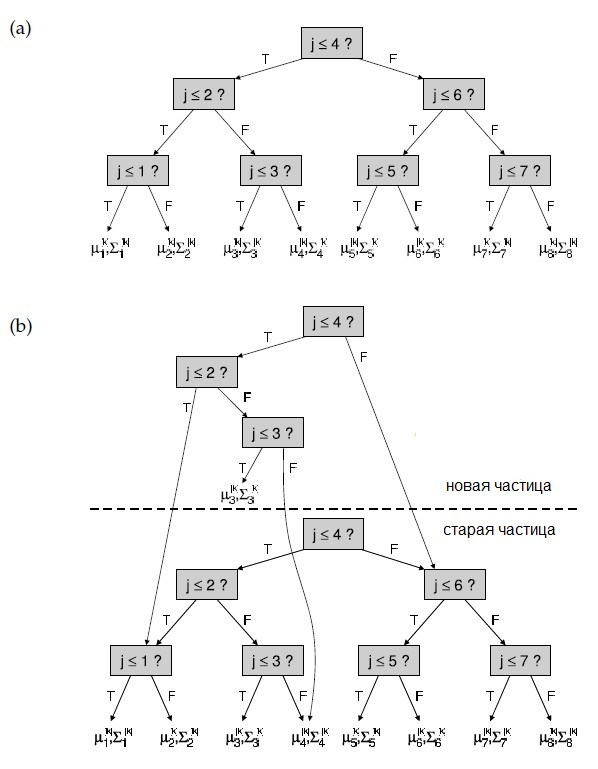
\includegraphics[width=0.95\linewidth]{138orig}}
	\caption{ ( Рис. 13.8    Дерево, выражающее $N=8$ оценок признаков в одной частице(a).
 Генерация новой частицы на основе старой, требует изменения лишь одного гауссиана (b). Новая частица получает лишь частичное дереве, состоящее из пути к измененному гауссиану. Все другие указатели копируются из генерирующего дерева, что может быть выполнено за время, логарифмически зависящее от $N$.) }
	\label{fig:138orig}
\end{figure}

\begin{figure}[H]
	\center{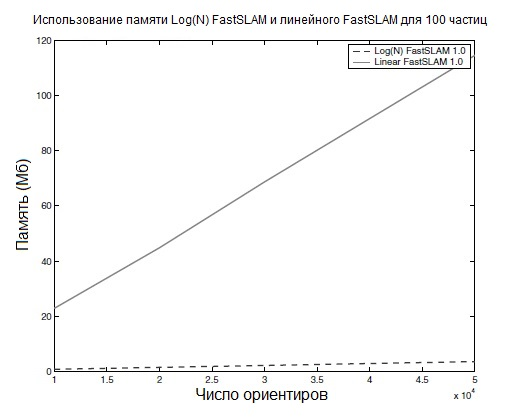
\includegraphics[width=0.8\linewidth]{139orig}}
	\caption{ ( Рис. 13.9 Требования памяти для линейной и логарифмической $\log(N )$ версии FastSLAM 1.0.) }
	\label{fig:139orig}
\end{figure}

Дерево позволяет существенно экономить память. На Рис. 13.9 показано влияние эффективной технологии отображения в виде дерева на требуемую для FastSLAM память. Этот граф является результатом реального использования FastSLAM 1.0 с $M=100$ частицами для получения карты на основе признаков. Согласно графу, для карты с 50000 признаков экономия составляет почти два порядка. Относительная экономия времени обновления имеет близкое значение.

Получение логарифмической сложности по времени для FastSLAM с неизвестной ассоциацией данных более трудно. Потребуется метод ограничения поиска ассоциации данных локальной окрестностью признака, чтобы предотвратить циркуляцию вероятности ассоциации данных для всех $N$ признаков карты. Кроме того, дерево должно оставаться приблизительно сбалансированным.

Конечно, существуют варианты деревьев ядерной оценки плотности (kernel density trees, kd-trees), способные удовлетворять этим требованиям, подразумевая, что дисперсия измерений датчика по сравнению с общим размером карты мала. Например, \textit{bkd-дерево} предложенное Прокопюк (Procopiuc et al., 2003), сохраняет последовательность деревьев возрастающей сложности. Путём последовательного смещения элементов по этим деревьям можно гарантировать амортизационное логарифмическое время вызова для вставки новых признаков в карту. Другим алгоритмом является DP-SLAM, предложенный Елизаром и Парром (Eliazar and Parr, 2003), в котором для эффективного хранения и получения используются \textit{деревья истории}, похожие на описанные.\\

\textbf{13.9	FastSLAM для карт на основе признаков}\\

\textbf{13.9.1	Эмпирические наблюдения}\\

Алгоритм FastSLAM применялся для большого количества выражений карт и данных датчиков. Наиболее общий вариант использования основан на картах признаков, считая, что робот оснащён датчиком для обнаружения расстояния и угла направления на ориентиры. Один из таких наборов данных, парк Виктории, уже обсуждался в Главе 12. На Рис. 13.10a показан путь робота на основе оценок управляющего воздействия.  Управляющие воздействия плохо прогнозируют местоположение транспорта, после 30 минут движения оценочное местоположение автомобиля более чем на 100 метров отличалось от положения по GPS.

На оставшихся трёх врезках на Рис. 13.10 показан итог работы FastSLAM 1.0. На всех схемах путь по GPS показан пунктиром, а результат работы FastSLAM – сплошной линией. Среднекадратичная ошибка результирующего пути составляет чуть больше 4 метров для перемещения длиной 4. Этот эксперимент проводился с числом частиц $M=100$. Эта ошибка практически не отличается от ошибки других наиболее совершенных алгоритмов SLAM, обсуждаемых в предыдущих главах. Надёжность FastSLAM становится очевидным из Рис. 13.10d, на котором приводится результат эксперимента, в котором информация о движении просто игнорировалась. Вместо этого, модель движения на основе одометрии была заменена броуновской моделью движения. Средняя ошибка FastSLAM статистически неотличима от ошибки, полученной ранее.

При реализации FastSLAM в картах на основе признаков важно учитывать отрицательную информацию. Когда отрицательная информация используется для оценки вероятности существования каждого признака, как описано в подразделе 13.6, многие ошибочные признаки на карте можно удалить. На Рис. 13.11 показана карта парка Виктория с учётом отрицательной информации и без него. Здесь использование отрицательной информации привело к уменьшению количества признаков результирующей карты на 44\% . Хотя истинное количество признаков недоступно, даже при беглом взгляде на карты видно, что множество ошибочных признаков было отброшено.

Имеет смысл сравнить FastSLAM с EKF SLAM, который остаётся популярным эталонным алгоритмом. Например, на Рис. 13.12 приводится сравнение точности FastSLAM 1.0 с EKF для различного числа частиц от 1 до 5000. Для сравнения ошибка EKF SLAM  показана пунктирной горизонтальной линией на Рис. 13.12. Точность FastSLAM 1.0 достигает точности EKF по мере увеличения количества частиц, и становится статистически неотличима после, приблизительно, 10 частиц. Это интересно уже потому, что FastSLAM 1.0 с 10 и 100 частицами требует на порядок меньше параметров, чем EKF SLAM для достижения аналогичного уровня точности.

\begin{figure}[H]
	\center{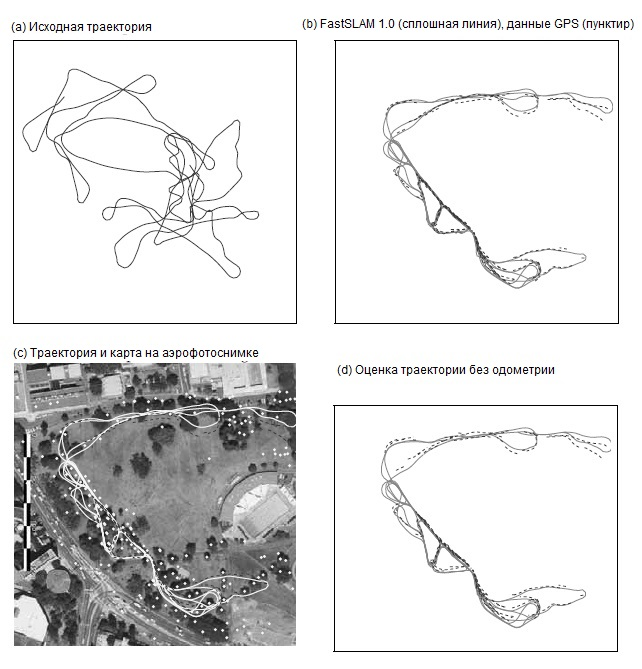
\includegraphics[width=1\linewidth]{1310orig}}
	\caption{ ( Рис. 13.10  Путь автомобиля на основе одометрии (a);  Реальный путь (показан пунктиром) и путь согласно FastSLAM 1.0 (сплошная линия) (b);  результаты обработки датасета наложенные на аэрофотосъемку, где путь согласно GPS показан синим (пунктиром), усреднённый путь FastSLAM 1.0 показан желтым (сплошная линия), а оценённые признаки показаны жёлтыми кругами (c). Набор данных созданный без информации об одометрии(d). Данные и аэрофотография принадлежат Хосе Гюванту и Эдуарду Неботу, австралийский центр полевой робототехники (José Guivant and Eduardo Nebot, Australian Centre for Field Robotics).) }
	\label{fig:1310orig}
\end{figure}

\begin{figure}[H]
	\center{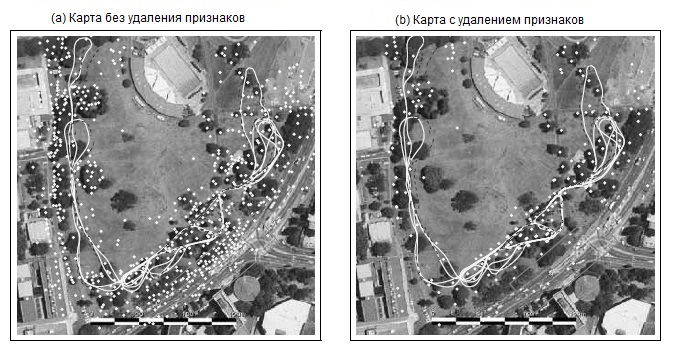
\includegraphics[width=0.9\linewidth]{1311orig}}
	\caption{ ( Рис. 13.11 FastSLAM 1.0 (a) без удаления признаков (b) с удалением признаков на основе отрицательной информации.) }
	\label{fig:1311orig}
\end{figure}

На практике, FastSLAM 2.0 даёт лучшие результаты по сравнению FastSLAM 1.0, хотя улучшение существенно только при определённых обстоятельствах. Как правило, результаты обоих алгоритмов сравнимы при большом числе частиц $M$ и когда шум измерений велик по сравнению с неопределённостью движения. Это показано на Рис. 13.13, где изображена точность каждого варианта FastSLAM в виде функции шума измерения, используя $M=100$ частиц. Наиболее важное наблюдение состоит в сравнительно низкой эффективности FastSLAM 1.0 в экспериментах с малошумными датчиками. Одним из способов проверить, страдает ли реализация FastSLAM 1.0 от этой проблемы, является искусственное увеличение шума измерений в вероятностной модели $p(z|x)$. Если в результате такого увеличения ошибка уменьшается, время переключиться на FastSLAM 2.0.

\begin{figure}[H]
	\center{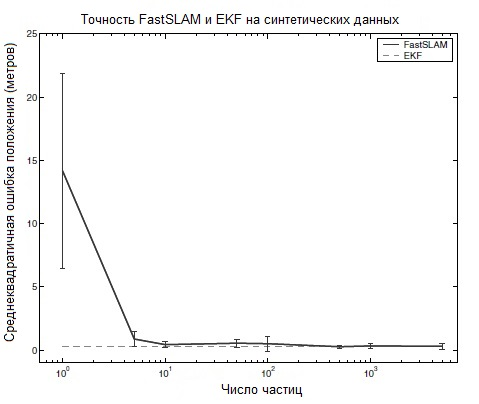
\includegraphics[width=0.6\linewidth]{1312orig}}
	\caption{ ( Рис. 13.12 Сравнительная точность FastSLAM 1.0 и EKF на синтетических данных.) }
	\label{fig:1312orig}
\end{figure}

\textbf{13.9.2	Замыкание цикла}\\

Совершенных алгоритмов не существует. Есть задачи, в которых FastSLAM проигрывает конкурентам на основе гауссовых моделей.  Одна из таких задач включает \textit{замыкание цикла}. В замыкании цикла робот движется через неизвестную территорию, и в некоторой точке, сталкивается с признаками, которые не были видны долгое время. Сохранение корреляции в алгоритме SLAM оказывается важным, поэтому информация, полученная при закрытии цикла, может распространяться через всю карту. EKF и GraphSLAM напрямую сохраняют такие корреляции, а FastSLAM сохраняет их с помощью разнообразия в наборах частиц. Поэтому, возможность замыкания циклов зависит от числа частиц $M$. Лучшее разнообразие в наборе элементов выборки приводит к лучшим показателям при замыкании циклов, поскольку новые наблюдения влияют на положение робота дальше в прошлом.

К сожалению, при обрезке неправильных траекторий робота, перевыборка однажды вызывает ситуацию, когда все частицы FastSLAM разделяют общую историю, начиная с некоторой точки в прошлом. Новые наблюдения неспособны повлиять на признаки, наблюдаемые до определённого момента. Общая точка истории может быть отодвинута назад во времени путём увеличения количества частиц $M$. Такой процесс отбрасывания данных корреляции со временем позволяет FastSLAM эффективно выполнять обновление датчика. Эта эффективность даётся ценой меньшей скорости сходимости. Отбрасывание информации корреляции означает, что для достижения заданного уровня точности требуется больше наблюдений. Очевидно, улучшенное предположительное распределение FastSLAM 2.0 гарантирует, меньшее количество уничтоженных частиц  при перевыборке в сравнении с FastSLAM 1.0, но  в решении проблемы это не поможет.

\begin{figure}[H]
	\center{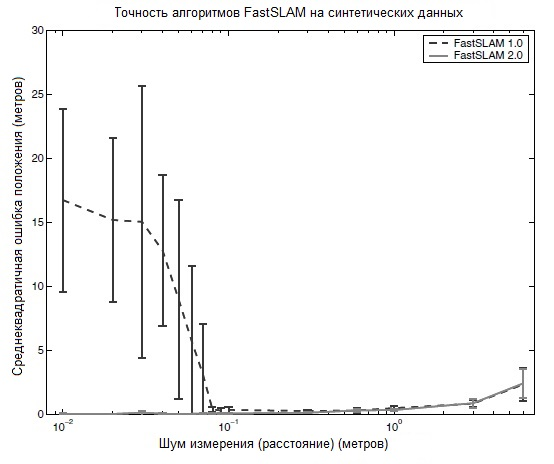
\includegraphics[width=0.65\linewidth]{1313orig}}
	\caption{ ( Рис. 13.13 FastSLAM 1.0 и 2.0 с разным уровнем шумов измерений: Как и ожидалось, FastSLAM 2.0 практически равномерно превосходит FastSLAM 1.0. Разница особенно очевидна для малых наборов частиц, где улучшенное предположительное распределение значительно лучше фокусирует частицы.) }
	\label{fig:1313orig}
\end{figure}

На практике, разнообразие важно, и стоит уделить внимание оптимизации алгоритма для поддержания максимального разнообразия. Примеры замыкания цикла показан на Рис. 13.15. На схемах приводятся истории всех $M$ частиц. На Рис. 13.15a частицы FastSLAM 1.0 имеют общую часть истории вокруг цикла. Новые наблюдения неспособны повлиять на положение признаков, наблюдаемых до порога. В случае FastSLAM 2.0 алгоритм в состоянии поддерживать разнообразие распространяя до начала цикла. Это критично для надёжного замыкания цикла и быстрой сходимости.

На Рис. 13.16a показан результат эксперимента по сравнению эффективности по замыканию цикла в FastSLAM 1.0 и 2.0. по мере увеличения размера цикла ошибка обоих алгоритмов возрастает. Однако, FastSLAM 2.0 стабильно превосходит FastSLAM 1.0. Этот же результат можно перефразировать в терминах частиц. FastSLAM 2.0 требует меньше частиц для закрытия данного цикла FastSLAM 1.0.

\begin{figure}[H]
	\center{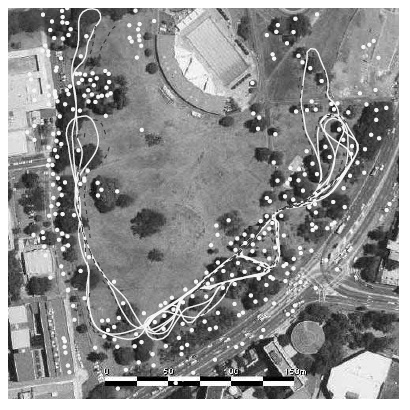
\includegraphics[width=0.65\linewidth]{1314orig}}
	\caption{ ( Рис. 13.14    Карта парка Виктории, созданная FastSLAM 2.0 с $M=1$ частицей.) }
	\label{fig:1314orig}
\end{figure}

На Рис. 13.16b показаны результаты эксперимента сравнения скорости сходимости FastSLAM 2.0 и EKF. FastSLAM 2.0 (с 1, 10 и 100 частиц) и EKF были запущены по 10 раз на большом имитационном цикле признаков, похожим на показанный на Рис. 13.16a и b. Для каждого запуска были использованы различные начальные параметры, вызывая генерацию различных наблюдений и управляющих воздействий в каждом цикле. Среднеквадратичная ошибка местоположения на карте на каждом такте времени была усреднена по 10 запускам для каждого алгоритма.

По мере перемещения робота по карте ошибка постепенно возрастает. Когда робот замыкает цикл на итерации 150, пересмотр старых признаков должен влиять на местоположение всех признаков вокруг цикла, вызывая уменьшение общей ошибки карты. Очевидно, так происходит с EKF. FastSLAM 2.0 с единственной частицей неспособен повлиять на местоположение прошлых признаков, поэтому ошибка признака не уменьшается. По мере добавления частиц к FastSLAM 2.0 фильтр способен применять данные наблюдений к местоположению признаков для прошлых моментов времени, постепенно достигая скорости сходимости EKF. Очевидно, количество частиц, необходимых для достижения времени сходимости, близкого к EKF, будет возрастать с размером цикла. Недостаток долговременных корреляций в выражении FastSLAM, пожалуй, наиболее важный недостаток в сравнении с методами SLAM на основе гауссовых представлений.

\begin{figure}[H]
	\center{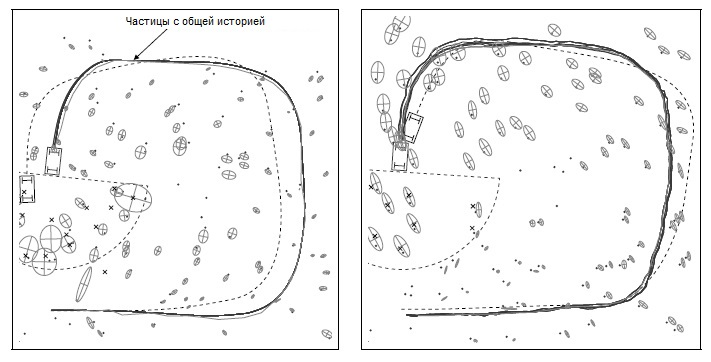
\includegraphics[width=0.8\linewidth]{1315orig}}
	\caption{ ( Рис. 13.15 FastSLAM 2.0 может закрывать циклы большего размера, чем FastSLAM 1.0 при постоянном количестве признаков.) }
	\label{fig:1315orig}
\end{figure}

\textbf{13.10	FastSLAM на основе сетки}\\

\textbf{13.10.1	Алгоритм}\\

В Главе 9 были изучены \textit{карты сеток занятости} как объёмное выражение окружающей среды робота. Преимуществом такого выражения является то, что для них не требуется предопределённых определений ориентиров. Вместо этого, можно моделировать произвольные типы сред. В оставшейся части главы будет выполнено обобщение FastSLAM  для таких представлений сред.

Для адаптации алгоритма FastSLAM к картам сеток занятости, понадобится три функции, уже определённые в предыдущих разделах. Во-первых, необходимо выполнить выборку из апостериорной вероятности движения $p(x_t|x_{t-1}^{[k]}, u_t)$ как в выражении 13.12. Для этого необходим метод выборки. Во-вторых, понадобится метод оценки карты для каждой частицы. Выяснилось, что мы можем полагаться на картографирование на основе сеток занятости, описанных в Главе 9. Наконец, требуется вычислить веса значимости отдельных частиц. Для этого необходим метод вычисления правдоподобия $p(z_t|x_t^k, m^{[k]})$ наблюдения $z_t$ зависящего от положения $x_t^k$, карты $m^{[k]}$, и самого последнего измерения $z_t$.

Как оказалось, обобщение FastSLAM для карт сеток занятости довольно очевидно. В Таблице 13.4 описан алгоритм FastSLAM с картами сеток занятости. Неудивительно, что в алгоритме присутствуют элементы локализации методом Монте-Карло (см. Таблицу 8.2) и картографирования на основе сеток занятости (см. Таблицу 9.1). Отдельные функции, используемые в алгоритме, являются вариантами аналогичных функций, применяемыми для локализации и картографирования.

\begin{figure}[H]
	\center{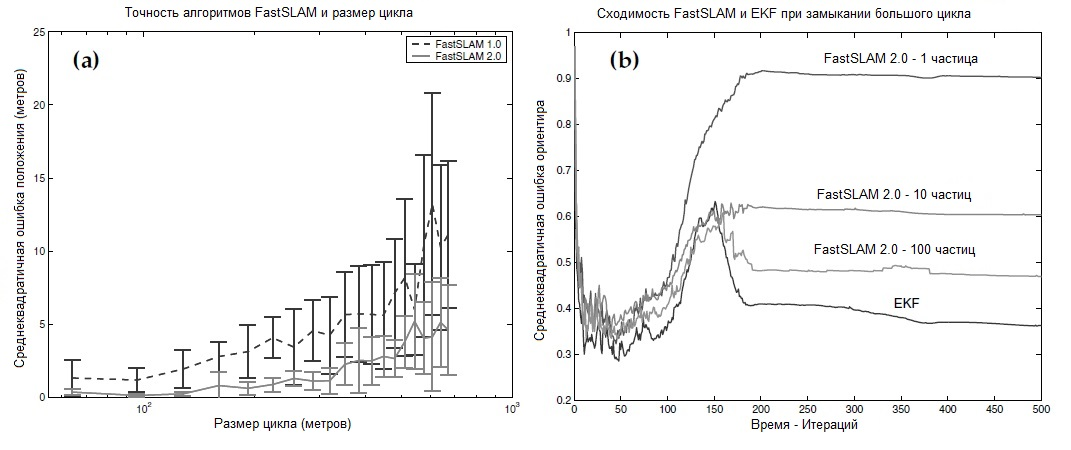
\includegraphics[width=1\linewidth]{1316orig}}
	\caption{ ( Рис. 13.16 Точность как функция размера цикла: FastSLAM 2.0 способен замыкать циклы большего размера, чем FastSLAM 1.0 при одинаковом количестве частиц (a).  Сравнение скорости сходимости FastSLAM 2.0 и EKF (b).) }
	\label{fig:1316orig}
\end{figure}

В частности, функция  \textbf{measurement\_model\_map}$(z_t,x_t^{[k]},m_{t-1}^{[k]})$
вычисляет правдоподобие измерения $z_t$ на основании положения $x_t^{[k]}$, выраженного $k$-й частицы и заданной картой $m_{t-1}^{[k]}$ предыдущего измерения и траекторией, выраженной этой частицей.   Далее, функция, \textbf{updated\_occupancy\_grid}$(z_t,x_t^{[k]},m_{t-1}^{[k]})$ вычисляет новую карту сетки занятости, на основании текущего положения $x_t^{[k]}$ $k$-ой частицы, связанной с ней карты $m_{t-1}^{[k]}$ и измерения $z_t$.

\textbf{13.10.2	Эмпирические соображения}\\

На Рис. 13.17 показана типичная ситуация использования алгоритма FastSLAM на основе сетки. Изображены три частицы со связанными с ними картами. Каждая частица выражает одну из потенциальных траекторий робота, что объясняет разницу карты сеток занятости. Центральная карта наилучшая с точки зрения глобальной целостности.

Типичная карта, полученная с помощью алгоритма FastSLAM, приведена на Рис. 13.19. Размер среды составляет 28 м$\times$28 м. Длина траектории робота составляет 491 м, а средняя скорость – 0,19 м/сек. Разрешение карты составляет 10 см. Для обучения этой карты было использовано всего 500 частиц. В течение всего процесса робот перемещался по двум циклами. Карта, вычисленная только на основе данных одометрии, показана на Рис. 13.18, где чётко видна величина погрешности одометрии робота. 

\begin{figure}[H]
	\center{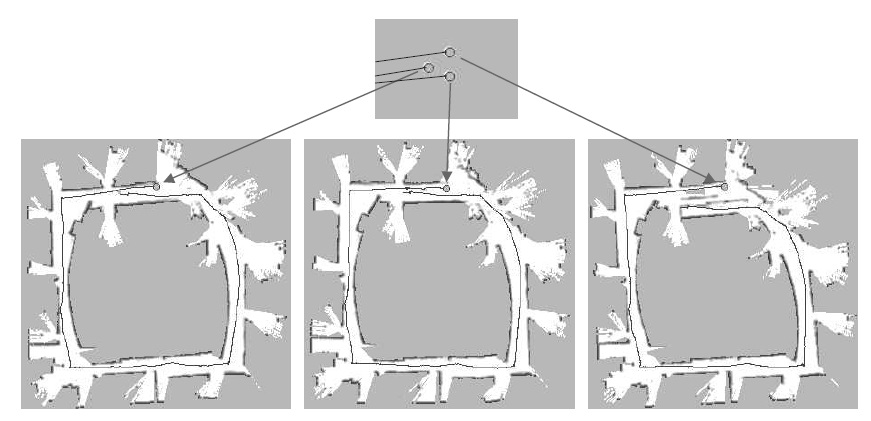
\includegraphics[width=1\linewidth]{1317orig}}
	\caption{ ( Рис. 13.17 Применение варианта алгоритма FastSLAM на основе сетки. Для каждой частицы имеется собственная карта, веса значимости части вычисляются на основе правдоподобия измерений, заданных собственными картами частицы.) }
	\label{fig:1317orig}
\end{figure}

\begin{figure}[H]
	\center{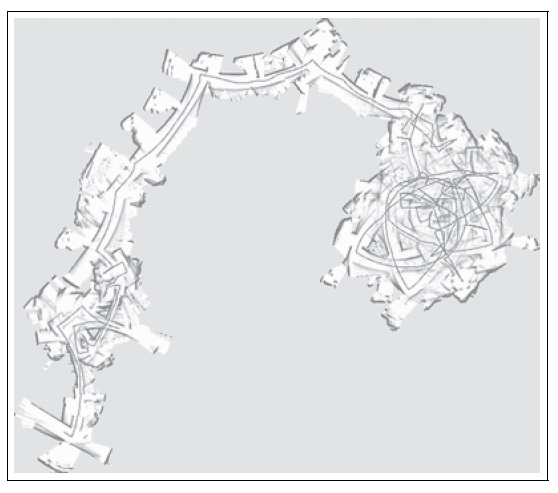
\includegraphics[width=0.8\linewidth]{1318orig}}
	\caption{ ( Рис. 13.18 Карта сетки занятости, сгенерированная из данных лазерного датчика расстояния и основанная только на одометрии. Все изображения принадлежат Дирку Хенелу, университет Фрайбурга (Dirk Hähnel, University of Freiburg).) }
	\label{fig:1318orig}
\end{figure}

\begin{figure}[H]
	\center{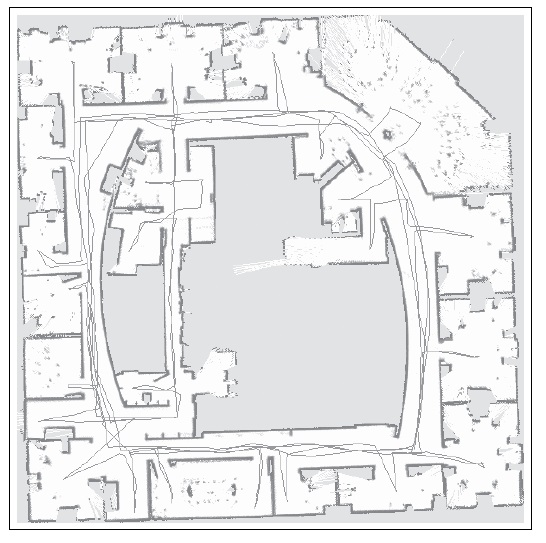
\includegraphics[width=0.8\linewidth]{1319orig}}
	\caption{ ( Рис. 13.19 Карта сетки занятости, соответствующая частице с наибольшим аккумулированным весом значимости, полученная алгоритмом, приведённым в Таблице 13.4 из данных, приведённых на Рис. 13.18. Количество частиц в этом эксперименте составляло 500. На рисунке также показан путь, выраженный частицей с максимальным аккумулированным весом значимости.) }
	\label{fig:1319orig}
\end{figure}

\begin{figure}[H]
	\center{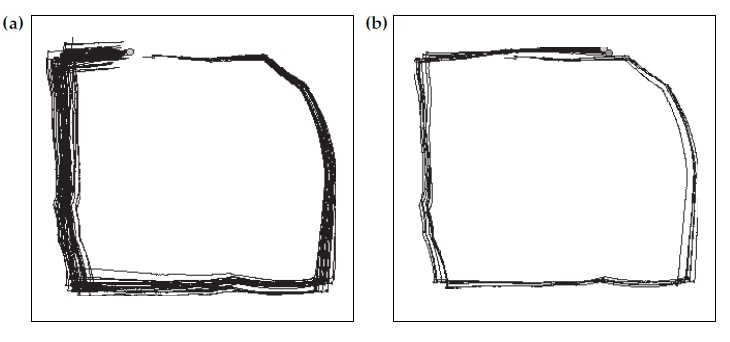
\includegraphics[width=1\linewidth]{1320orig}}
	\caption{ ( Рис. 13.20 Траектории по всей выборке перед (слева) и после (справа) замыкания внешнего цикла в среде, приведённой на Рис. 13.19. Изображения принадлежат Дирку Хенелу, университет Фрайбурга (Dirk Hähnel, University of Freiburg).) }
	\label{fig:1320orig}
\end{figure}

\begin{table}[H]
\begin{center}
\begin{tabular}{|l|}
\hline
{}\\
1:\textbf{ Algorithm FastSLAM\_occupancy\_grids}$(\mathcal{X}_{t-1},u_t,z_t):\qquad\qquad$\\
{}\\
2:\hspace{5mm}$ \bar{\mathcal{X}}_t=\mathcal{X}_t=\emptyset$\\
3:\hspace{5mm}$\textit{for}\,k=1\,\textit{to}\,M\,\textit{do}$\\
4:\hspace{10mm}$x_t^{[k]}=\textbf{sample\_motion\_model}\,(u_t,x_{t-1}^{[k]})$\\
5:\hspace{10mm}$w_t^{[k]}=\textbf{measurement\_model\_map}\,(z_t,x_t^{[k]},m_{t-1}^{[k]})$\\
6:\hspace{10mm}$m_t^{[k]}=\textbf{updated\_occupancy\_grid}\,(z_t,x_t^{[k]},m_{t-1}^{[k]})$\\
7:\hspace{10mm}$\bar{\mathcal{X}}_t=\bar{\mathcal{X}}_t+\langle x_t^{[k]},m_t^{[k]},w_t^{[k]}\rangle$\\
8:\hspace{5mm}$\textit{endfor}$\\
9:\hspace{5mm}$\textit{for}\,k=1\,\textit{to}\,M\,\textit{do}$\\
10:\hspace{9mm}$\textit{извлечь i с вероятностью}\,\propto\,w_t^{[i]}$\\
11:\hspace{9mm}$\textit{прибавить}\,\langle x_t^{[i]},m_t^{[i]}\rangle\,\textit{к}\,\mathcal{X}_t$\\
12:\hspace{5mm}$\textit{endfor}$\\
13:\hspace{5mm}$\textit{return}\,\,\mathcal{X}_t$\\
{}\\
\hline
\end{tabular}
\caption{(Таблица 13.4    Алгоритм FastSLAM для обучения карт сеток занятости.)}
\end{center}
\end{table}


Важность использования нескольких частиц становится очевидной на Рис. 13.20, иллюстрирующем траектории по выборке до и после замыкания цикла. Как видно на левом рисунке, положение робота достаточно неопределённо относительно начального, отсюда большой разброс к к моменту замыкания цикла. Однако, уже несколько шагов перевыборки после того, как робот оказался на уже знакомой территории, оказалось достаточно для значительного уменьшения неопределённости (правый рисунок).\\

\textbf{13.11	Выводы}\\

В этой главе был представлен метод многочастичного фильтра для решения задачи SLAM известный как алгоритм FastSLAM.\\

•	Основная идея FastSLAM состоит в сохранении набора частиц. В каждой частице путь робота содержится в виде выборки элементов. В ней также содержится карта, но каждый признак на карте выражается собственным локальным гауссианом. Результирующее выражение требует памяти, линейно зависящей от размера карта и количества частиц.\\

•	Основное преимущество представления карты в виде набора отдельных гауссиан, вместо одной общей функции, как для алгоритма EKF SLAM, возможно из-за факториальной структуры задачи SLAM. Было замечено, что признаки карты для данного пути условно независимы. Выполняя факторизацию по пути (по одному на частицу), можно просто считать каждый признак карты независимым, избежав затратный шаг сохранения корреляции между ними, который так вредит в методе EKF.\\

•	Обновление в FastSLAM напрямую повторяет обновление обычного многочастичного фильтра: выполняется выборка по новому положению, затем обновляются обнаруженные признаки. Это обновление может выполняться онлайн, а FastSLAM – служить решением онлайн задачи SLAM.\\

•	Далее, было замечено, что FastSLAM решает обе задачи SLAM: онлайн SLAM и оффлайн SLAM. В выводе FastSLAM считается оффлайн алгоритмом, в котором частицы представляют выборку в пространстве пути, а не только положений текущего момента. Однако. Оказывается, что ни для одного из шагов обновления не требуется знания положений, кроме текущего, поэтому оценки прежних положений можно отбросить. Это делает возможным запуск FastSLAM в виде фильтра. И предотвращает линейный рост размера частиц с увеличением карты.\\

•	Мы столкнулись с двумя вариантами FastSLAM, с номерами версий 1.0 и 2.0. FastSLAM 2.0 является расширенной версией FastSLAM. Он отличается от базовой версии одной ключевой идеей: FastSLAM 2.0 учитывает измерение при выборке нового положения. Математический вывод оказался несколько более сложным, но FastSLAM 2.0 превзошёл предшественника FastSLAM 1.0, поскольку ему требуется меньше частиц.\\

•	Идея использования многочастичных фильтров делает возможным удаление переменных ассоциации данных на основе частиц.   Каждая частица может основываться на разной ассоциации данных. Это даёт FastSLAM очевидный и мощный механизм решения проблем ассоциации данных в SLAM. Предыдущие алгоритмы, особенно EKF, GraphSLAM, и SEIF, могли использовать лишь единственное решение ассоциации данных для всего фильтра в произвольный момент времени, а значит, требовали большего внимания при выборе значения ассоциации данных.\\

•	Для эффективного обновления частиц со временем обсуждались отображения карты в виде дерева. Эти отображения позволили уменьшить сложность обновления FastSLAM с линейной до логарифмической, позволив разделение идентичных участков карты между частицами. Идеи таких деревьев важны на практике, поскольку позволяют масштабировать FastSLAM до $10^9$ или более признаков на карте.\\

•	Также обсуждались методы использования отрицательной информации. Один из них выполняет удаление с карты признаков, которые не поддерживаются существенными данными наблюдений. Здесь FastSLAM использует метод интеграции доказательств, знакомый с главы о картах сеток занятости. Другой касается взвешивания самих частиц. Если на карте частицы не удалось обнаружить искомую частицу путём измерения, значимость такой частицы может быть понижена умножением на соответствующий коэффициент.\\

•	Было обсуждено множество практических свойств двух алгоритмов FastSLAM. Эксперименты показали работоспособность обоих алгоритмов на практике, как для карт на основе признаков, так и для объёмных карт сеток занятости. С практической точки зрения, FastSLAM является одним из лучших вероятностных методов SLAM на текущий момент. Его возможности масштабирования сравнимы только с возможностями некоторых алгоритмов информационных фильтров, описанных в предыдущих двух главах.\\

•	Алгоритм FastSLAM 2.0 был обобщён для различных представлений карты. В одном из представлений карта состояла из точек, обнаруженных лазерным датчиком расстояния. В этом случае удалось отказаться от идеи моделировать неопределённость в признаках с помощью нормальных распределений и положиться на методы сравнения сканирований для реализации прямого процесса выполнения выборки в FastSLAM 2.0. Использование многочастичного фильтра дало надежный метод замыкания цикла.\\

Возможно, самым большим ограничением FastSLAM является неявная сохранение зависимости оценок местоположений признаков   
в виде разнообразия в наборе частиц. При определённых обстоятельствах это может негативно повлиять на скорость сходимости по сравнению с гауссовыми методами SLAM. При использовании FastSLAM следует предпринимать меры по уменьшению негативных эффектов истощения частиц в FastSLAM.\\

\textbf{13.12	Библиографические примечания}\\

Идея вычисления распределений по наборам переменных, комбинируя выборку с параметрической функцией плотности принадлежит Рао (Rao (1945) и Блеквеллу (Blackwell, 1947). Сегодня эта идея превратилась в общепринятый инструмент в литературе по статистике (Gilks et al. 1996; Doucet et al. 2001). Первый алгоритм картографирования на основе многочастичных фильтров для замыкания циклов был найден Труном (Thrun et al., 2000b). Формальное введение в многочастичные фильтры Рао-Блеквелла в области SLAM было выполнено Мерфи (Murphy, 2000a), Мерфи и Расселом (Murphy and Russell, 2001), разработавшими эту идею в контексте карт сеток занятости.

Алгоритм FastSLAM был впервые разработан Монтемерло (Montemerlo et al., 2002a), который также предложил выражения в виде деревьев для эффективного сохранения нескольких карт. Обобщение этого алгоритма для карт высокого разрешения было выполнено Елизаром и Парром, чей алгоритм DP-SLAM генерировал карты из показаний лазерного датчика расстояния с беспрецедентной на тот момент точностью и детализацией. Центральная структура данных называлась "деревья наследования", и расширяла деревья FastSLAM для обновления карт на основе сеток занятости. Более эффективная версия известна как DP-SLAM 2.0 (Eliazar and Parr 2004). Алгоритм FastSLAM 2.0 был разработан Монтемерло (Montemerlo et al., 2003b) и основан на предыдущей работе ван дер Мерве (van der Merwe et al., 2001), впервые предложившем идею использования измерения как части предполагаемого распределения в теории многочастичных фильтров. Алгоритм FastSLAM на основе сеток в этой главе принадлежит Хенелу (Hähnel et al., 2003b), который интегрировал идею улучшенного предполагаемого измерения с фильтрами Рао-Блеквелла, применимыми для карт на основе сеток. Фильтр Рао-Блеквелла для отслеживания состояния дверей в динамической офисной среде описан в работе Авотса (Avots et al., 2002).

Одним из наиболее важных вкладов в FastSLAM является область ассоциации данных, которой уделялось много внимания в литературе по SLAM. В оригинальной работа по SLAM (Smith et al. 1990; Moutarlier and Chatila 1989a)  ассоциация данных выполнялась методом максимального правдоподобия, как было детально выведено Диссанаяки (Dissanayake et al., 2001). Ключевым ограничением этих методов ассоциации данных была невозможность обеспечить взаимную исключительность: два разных признака в одном измерении датчика (или в течение короткого промежутке времени) не могут соответствовать одному и тому же физическому признаку окружающего мира. Воспользовавшись этом принципом, Ниера и Тардос разработали методы проверки соответствия для наборов признаков, позволившие уменьшить количество ошибок ассоциации данных. Чтобы адаптировать алгоритм к огромному количеству потенциальных ассоциаций (экспоненциальному к количеству признаков, учитываемых в каждый момент времени), Ниера (Neira et al., 2003) предложил методы случайной выборки в пространстве ассоциации данных. Однако, все эти методы сохраняли в апостериорном распределении SLAM только одну моду. Федер (Feder et al., 1999) применил идею жадной ассоциации данных к данным сонара, но реализовал отложенное решение для разрешения двойственности.

Идея сохранения многомодального апостериорного распределения в SLAM восходит к работам Дюррран – Уайта (Durrant-Whyte et al., 2001), в алгоритме которого используется смесь нормальных функций для выражения апостериорной вероятности. Каждый компонент смеси соответствует разному следу в истории всех решений ассоциации данных. FastSLAM тоже следует этой идее, но вместо смеси компонент гауссиан используются частицы. Идею ленивой ассоциации данных можно отследить до других областей, например, популярного алгоритма RANSAC (Fischler and Bolles 1981) в машинном зрении. Алгоритм дерева, представленный в предыдущей главе, был разработан Хенелом (Hähnel et al., 2003a). Как уже упоминалось, он основан на работах Куперса (Kuipers et al., 2004). Совершенно иной подход в ассоциации данных описан в работе Шаткай и Келблинга (Shatkay and Kaelbling, 1997), Труна (Thrun et al., 1998b), которые использовали алгоритм \textit{максимизации ожидания} для решения проблем соответствия (см. (Dempster et al. 1977)). Алгоритмы максимизации ожидания последовательно проходят такты ассоциации данных для всех признаков в фазе построения карты, таким, образом, одновременно выполняя поиск в пространстве численных параметров карты и дискретном пространстве соответствий. Аранеда (Araneda, 2003) успешно использовал методы MCMC для ассоциации данных в оффлайн SLAM.

Проблема ассоциации данных естественно возникает в контексте интеграции карт нескольких роботов. В большом количестве разработок были представлены алгоритмы для локализации одного робота относительно другого, допуская, что оба работают в одной среде, а их карты пересекаются (Gutmann and Konolige 2000; Thrun et al. 2000b). Рой и Дудек (Roy and Dudek, 2001) разработали метод, в котором для интеграции информации роботам необходимо сблизиться. В общем случае, однако, метод ассоциации данных должен учитывать возможность того, что карты не пересекаются. Стюарт (Stewart et al., 2003) разработал алгоритм многочастичного фильтра, явно моделирующего возможность непересекающихся карт. В их алгоритме для вычисления вероятности наличия в среде «общих» локальных карт использована байесовская оценочная функция. Идея наложения множеств признаков для ассоциации данных в картографировании с помощью нескольких роботов принадлежит Дедеоглу и Сухаттме (Dedeoglu and Sukhatme, 2000), а также Труну и Лю (Thrun and Liu, 2003). Новое неплоское выражение карт было предложено Говардом (Howard, 2004), и позволило избежать потери целостности в неполных картах. Его метод позволил получить весьма точные результаты картографирования несколькими роботами (Howard et al. 2004).\\

\textbf{13.13	Упражнения}\\

1.	Назвать три ключевых, явных преимуществ каждого из алгоритмов SLAM: EKF, GraphSLAM и FastSLAM.\\

2.	Описать обстоятельства, при которых FastSLAM 1.0 не будет сходиться, а FastSLAM 2.0 сойдётся к точной карте (с вероятностью 1).\\

3.	На странице 443 ???, было указано, что \textit{зависимости от самого положения $x_t$ вместо всего пути $x_{1:t}$ недостаточно, поскольку зависимости могут возникнуть в предыдущих положениях.} Доказать это утверждение, можно на примере.\\

4.	FastSLAM генерирует множество различных карт, по одной для каждой частицы. Вопрос комбинирования таких карт в единую апостериорную карту остался открытым в этой главе. Предложить два метода, один для FastSLAM с известным соответствием, и один для FastSLAM с ассоциацией данных для каждой частицы.\\

5.	Преимущество FastSLAM 2.0 над FastSLAM 1.0 заключается в природе предполагаемого распределения. Разработать аналогичное распределение для локализации методом Монте-Карло: Вывести похожее предполагаемое распределение для MCL в картах на основе признаков, и включить в результирующий алгоритм “MCL 2.0.” Для этого упражнения может понадобиться допущение об известном соответствии.\\

6.	В подразделе 13.8 описана эффективная реализация в виде дерева, но псевдокод не приведён. В этом упражнении требуется описать соответствующие структуры данных и уравнения обновления для дерева, считая, что количество признаков заранее известно, а необходимости обрабатывать проблему соответствия нет.\\

7.	В этом задании требуется эмпирически проверить, что FastSLAM действительно сохраняет корреляции между оценками признаков и оценкой положения робота. Требуется разработать простой алгоритм Fast- SLAM 1.0 для линейного гауссового SLAM. Можно вспомнить из предыдущих упражнений уравнения движения и измерения в линейном гауссовом SLAM с аддитивным гауссовым шумом:\\

$x_t\sim\mathcal{N}(x_{t-1}+u_t,R)$\\

$z_t=\mathcal{N}(m_j-x_t,Q)$\\

Запустить FastSLAM 1.0 в симуляторе. После $t$ шагов, обучить гауссову функцию в объединённому пространстве местоположений признаков и положению робота. Вычислить матрицу корреляции на основании этого гауссиана и охарактеризовать степень корреляции как функцию по $t$. Что показали наблюдения?\\

8.	Как упоминалось в тексте, FastSLAM является многочастичным фильтром Рао-Блеквелла. В этом упражнении требуется разработать фильтр Рао-Блеквелла для другой задачи – локализации робота, которого систематически заносит в сторону. Систематический занос является общим явлением в одометрии – обратите внимание на Рис. 9.1 и 10.7 где показаны довольно явные проявления заноса. Допустим, дана карта среды. Можно ли разработать фильтр Рао-Блеквелла, который одновременно оценивает параметры заноса робота и глобальное местоположение робота в среде? В предлагаемом фильтре следует комбинировать многочастичные фильтры и фильтры Калмана.\\






 
\end{document}